% An example latex source file for your reports
%
% Do NOT alter from here to "\begin{document}"

\documentclass[12pt,usenames,dvipsnames]{article}
\usepackage[left=2.3cm,top=2.3cm,right=2.3cm,bottom=2.3cm,marginparwidth=1cm]{geometry}
\usepackage{siunitx}
\usepackage{gensymb}
\usepackage{amsfonts}
\usepackage{amsmath}
\usepackage{amssymb}
\PassOptionsToPackage{hyphens}{url}\usepackage[colorlinks=true,linkcolor=blue,urlcolor=blue]{hyperref}
\usepackage{mathtools} % required for $\coloneqq$
\pagenumbering{arabic}
\usepackage{appendix}
\usepackage{indentfirst}
\usepackage{caption}
\usepackage{subcaption}
\usepackage{needspace}
\usepackage{amsmath}
\usepackage{cleveref}
\usepackage[most]{tcolorbox}
\usepackage[demo]{graphicx}
\usepackage{sidecap}   
\usepackage[toc,page]{appendix}
\usepackage[english]{babel}
\usepackage{graphicx}
\usepackage{subcaption}
\newtcbtheorem{Theorem}{Theorem}{
  enhanced,
  sharp corners,
  attach boxed title to top left={
    yshifttext=-1mm
  },
  colback=white,
  colframe=blue!50!black,
  fonttitle=\bfseries,
  boxed title style={
    sharp corners,
    size=small,
    colback=blue!50!black,
    colframe=blue!50!black,
  } 
}{thm}

\newtcbtheorem{Definition}{Definition}{
  enhanced,
  sharp corners,
  attach boxed title to top left={
    yshifttext=-1mm
  },
  colback=TealBlue!3,
  colframe=blue!50!black,
  fonttitle=\bfseries,
  boxed title style={
    sharp corners,
    size=small,
    colback=blue!50!black,
    colframe=blue!50!black,
  } 
}{def}

\newtcbtheorem{Corollary}{Corollary}{
  enhanced,
  sharp corners,
  attach boxed title to top left={
    yshifttext=-1mm
  },
  colback=TealBlue!3,
  colframe=blue!50!black,
  fonttitle=\bfseries,
  boxed title style={
    sharp corners,
    size=small,
    colback=blue!50!black,
    colframe=blue!50!black,
  } 
}{def}

\bibliographystyle{unsrt}
\begin{document}

% CHANGE THE FOLLOWING INFORMATION:

\begin{center}
  \large\textbf{Two-Body Problem and Restricted Three-Body Problem} \\
  10th June, 2022 \\
  Eason Li
\end{center}

\nocite{AngularMomentum:2016, 99MurraySolarSys, CURTIS2014xi, John2005, Matplotlib, odeint, ZMBQ2014}

\section{Introduction}

Observing, exploring, and ultimately understanding our solar system is the first step towards understanding the rest of the universe. The key discovery in this process was Newton’s formulation of the universal law of gravitation; this made sense of the orbits of planets, satellites, and comets, and their future motion could be predicted: The Newtonian universe was a deterministic system. However, advances in mathematics and computer technology have now revealed that, even though our system is deterministic, it is not necessarily predictable. The study of nonlinear dynamics has revealed a solar system even more intricately structured than Newton could have imagined. ~\cite{99MurraySolarSys}.

To begin to explore our solar system and the gigantic universe, we need to introduce you several theories:

\subsection{Kepler's Laws of Planetary Motion}
\label{Kepler's Laws}
The Kepler's Laws of Planetary Motion are described as following: \\

1) The planets move in ellipses with the Sun at one focus.

2) A radius vector from the Sun to a planet sweeps out equal areas in
equal times.\label{Kepler Second Law}

3) The square of the orbital period of a planet is proportional to the cube of its semi-major axis. \\

Kepler’s third law relates a, the half of the length of the major axis of an ellipse, to the period $T$ of the planet’s orbit. He deduced that $T^2 \propto a^3$, so that if two planets have semi-major axes $a_1$ and $a_2$ and periods $T_1$ and $T_2$, then 
\begin{equation}
    \frac{T_a}{T_2} = (\frac{a_1}{a_2})^{3/2}
\end{equation}
which is consistent with his original formulation of the law. 

\subsection{Newton's Universal Laws of Gravitation}
In scalar form, Newton proposed that the magnitude of the force $F_g$ between any two masses in the universe, $m_1$ and $m_2$, separated by a distance $r$ is given by
\begin{equation}
F_{g} = G\frac{m_{1}m_{2}}{r^2}
\label{eq:unigrav}
\end{equation}

where $G$ is the gravitational constant.

\section{Two-Body Problem}

\subsection{Introduction to the Two-Body Problem}
Two-Body Problem is considered to be the easiest, predictable problem among all the N-Body Problems, and it can be found everywhere in the universe, which indispensably exists in our solar system. It concerns the interaction of two point masses moving under a mutual gravitational attraction described by Newton's Universal Law of Gravitation, Eq.~\ref{eq:unigrav}.

In this chapter we derive the basic equations of planetary motion and solve the two-body problem, showing how Kepler’s laws arise.

\subsection{Equations of Motion}
Considered the motion of two masses $m_{1}$ and $m_{2}$ with position vectors $\bf{r_1}$ and $\bf{r_2}$ with respect to some fixed origin in inertial space. (See figure 1 above)

\begin{figure}
    \centering
    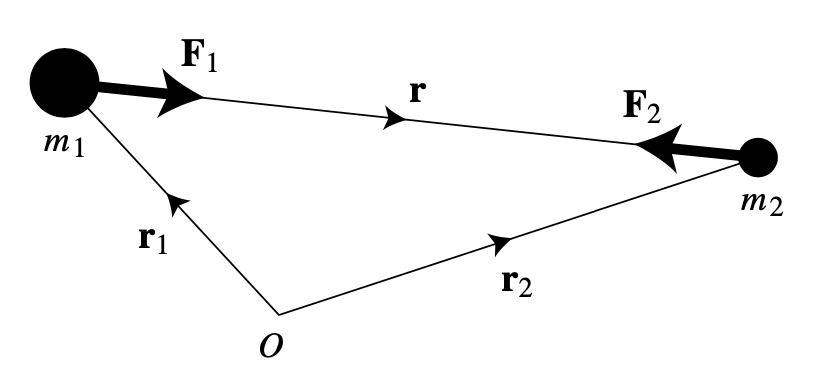
\includegraphics{masses, vectors.png}
    \caption{A vector diagram for the forces acting on two masses, m1 and m2, with position vectors $\bf{r_1}$ and $\bf{r_2}$.}
    \label{fig:masses vectors}
\end{figure}

We can easily find that $\bf{r} = \bf{r_2} - \bf{r_1}$, which the vector $\bf{r}$ denotes the relative position of the mass $m_2$ with respect to $m_1$. Remember we have the formula for force and gravitational force:
\begin{equation}
    Force ~Formula: \vec{F} = m \times \vec{a}
\end{equation}
\begin{equation}
    Gravitational ~Force ~Formula: \vec{F_{g}} = G \frac{m_{1}m_{2}}{r^2}
\end{equation}
Apply them to our situation, the net force acting on $m_1$ is:
\begin{equation}
    \vec{F_{1}} = G\frac{m_{1}m_{2}}{r^2} \times \frac{\bf{r}}{\left| r \right|} = m_{1}\bf{\ddot{r}_{1}}
    \label{eq:force on m1}
\end{equation}
the net force acting on $m_2$ is:
\begin{equation}
    \vec{F_{2}} = -G\frac{m_{1}m_{2}}{r^2} \times \frac{\bf{r}}{\left| r \right|} = m_{2}\bf{\ddot{r}_{2}}  
    \label{eq:force on m2}
\end{equation}
From Newton's Third Law, we know that if an object A exerts a force on object B, then object B must exert a force of equal magnitude and opposite direction back on object A. In the scenario we have, the only force acting on each mass is the gravitational force exerted from another, so that:
\begin{equation}
    \vec{F_1} + \vec{F_2} = 0,
\end{equation}
which is equivalent to:
\begin{equation}
    m_{1} {\bf{\ddot{r}}_{1}} + m_{2} {\bf{\ddot{r}}_2} = 0
    \label{eq:newton's third law}
\end{equation}
Integrate equation (\ref{eq:newton's third law}) on both sides we can get:
\begin{equation}
    m_{1} {\bf{\dot{r}}_{1}} + m_{2} {\bf{\dot{r}}_2} = {\bf{c_1}}
    \label{eq:first degree integration}
\end{equation}
Integrating equation (\ref{eq:first degree integration}) on both sides gives us:
\begin{equation}
    m_{1} {\bf{r}_{1}} + m_{2} {\bf{r}_2} = {\bf{c_1}} t + {\bf{c_2}},
    \label{eq:second degree integration}
\end{equation}
where $\bf{c_1}$ and $\bf{c_2}$ are both constant vectors.

\begin{Definition}{Centre of Mass}{}
    The coordinates of, $R$, the centre of mass of a system of particles is represented by the formula:
    \begin{equation}
        {\bf{R}} = \frac{1}{M} \sum_{i=1}^{n}m_{i}{\bf{r_{i}}},
    \end{equation}
    where $M = \sum_{i=1}^{n}m_{i}$ is the total mass of all the particles in the system. 
\end{Definition}

Using the definition of the centre of mass, and using the equations (\ref{eq:second degree integration}) and (\ref{eq:first degree integration}), we can now find the centre of mass of $m_{1}$ and $m_{2}$ in our case:
\begin{equation}
    {\bf{\dot{R}}} = \frac{{\bf{c_1}}}{m_{1}+m_{2}}~~~~~and~~~~~{\bf{R}} = \frac{{\bf{c_1}}t+{\bf{c_2}}}{m_{1}+m_{2}}
\end{equation}

This implies that either the centre of mass is stationary (if ${\bf{c_1}}=0$), or it is moving with a constant velocity in a straight line with respect to the origin O.

We consider the system of the two masses as stationary, or the centre of mass of $m_1$ and $m_2$ is motionless, so we can obtain the system of equations:
\begin{equation}
    \begin{cases}
        m_1 \mathbf{r_1} + m_2 \mathbf{r_2} = 0\\
        \mathbf{r_2 - r_1 = r}
    \end{cases}
\end{equation}
Solving for the system of equations we can get:
\begin{equation}
    \begin{cases}
        \mathbf{r_1} = \frac{-m_2 \mathbf{r}}{m_1 + m_2}\\
        \mathbf{r_2} = \frac{m_1 \mathbf{r}}{m_1 + m_2},
    \end{cases}
\end{equation}
which means that we are able to get $\mathbf{r_1}$ and $\mathbf{r_2}$ by just finding $\mathbf{r}$.\\\\

Now let us consider the motion of $m_{2}$ with respect to $m_{1}$. We already know that ${\bf{r} = {\bf{r_2}}} - {\bf{r_1}}$, this yields us:
\begin{equation}
    {\bf{\ddot{r}}} = {\bf{\ddot{r}}}_{2} - {\bf{\ddot{r}}}_{1} ~~ \Rightarrow{} ~~ {\bf{\ddot{r}}} + {\bf{\ddot{r}}}_{1} - {\bf{\ddot{r}}}_{2} = 0
    \label{eq:13}
\end{equation}
and using the equations (\ref{eq:force on m1}) and (\ref{eq:force on m2}), we can obtain:
\begin{equation}
    {\bf{\ddot{r}}}_1 = \frac{\vec{F}_{1}}{m_1} = \frac{G\frac{m_{1}m_{2}}{r^3}\vec{r}}{m_1} = \frac{Gm_{2}\vec{r}}{r^3} ~~~~~ and ~~~~~ {\bf{\ddot{r}}}_2 = \frac{\vec{F}_{2}}{m_2} = \frac{-G\frac{m_{1}m_{2}}{r^3}\vec{r}}{m_2} = \frac{Gm_{1}\vec{r}}{r^3}
    \label{eq:vector r1 and r2}
\end{equation}
We substitute the two expressions from (\ref{eq:vector r1 and r2}) into equation (\ref{eq:13}):
\begin{equation}
    \frac{{d^2}{\bf{r}}}{dt^2} + \frac{Gm_{2}\vec{r}}{r^3} - \frac{-Gm_{1}\vec{r}}{r^3} = 0
\end{equation}
Further simplify the equation, we can get:
\begin{equation}
    \frac{{d^2}{\bf{r}}}{dt^2} + G(m_{2}+m_{1})\frac{\vec{r}}{r^3} = 0,
    \label{eq:equation of relative motion}
\end{equation}
where the equation (\ref{eq:equation of relative motion}) is the equation of relative motion.

In order to solve it and find the path of $m_2$ relative to $m_1$ we must first derive several constants of the motion.

Taking the vector product of {\bf r} with equation (\ref{eq:equation of relative motion}) we have:
\begin{equation}
    {\bf r} \times {\bf{\ddot{r}}} = 0
    \label{eq:17}
\end{equation}

\begin{figure}
    \centering
    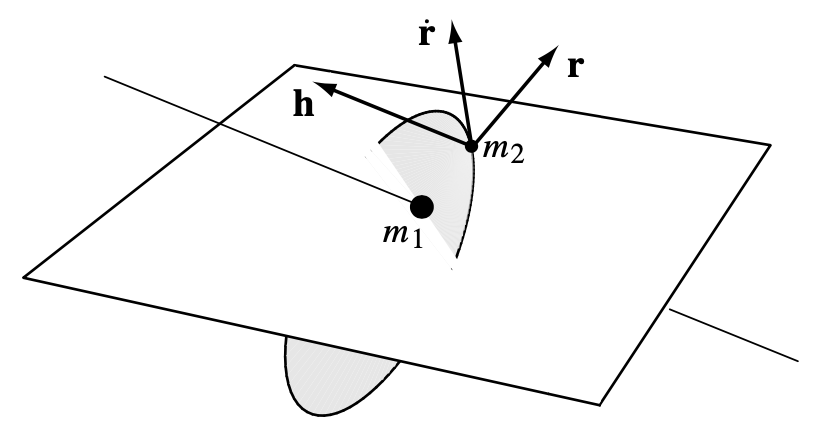
\includegraphics{motion of m2 with respect to m1.png}
    \caption{The motion of $m_2$ with respect to $m_1$ defines an orbital plane (the shaded region), because ${\bf r}\times{\bf{\dot{r}}}$, the cross product, is a constant vector, ${\bf h}$, the angular momentum vector, and this is always perpendicular to the orbit plane.}
    \label{fig:motion of m2 with respect to m1}
\end{figure}

\begin{Corollary}{Derivative of ${\bf r}\times{\bf{\dot{r}}}$}{}
    \begin{equation}
        \frac{d}{dt}({\bf r}\times{\bf{\dot{r}}}) = {\bf{r}}\times{\bf{\ddot{r}}}
    \end{equation}
    \label{corollary 1}
\end{Corollary}
proof: 
\begin{equation}
    \frac{d}{dt}({\bf r}\times{\bf{\dot{r}}}) = {\bf\dot{r}}\times{\bf{\dot{r}}} + {\bf r}\times{\bf{\ddot{r}}} = 0 + {\bf r}\times{\bf{\ddot{r}}} = {\bf r}\times{\bf{\ddot{r}}}
\end{equation}
Using above Corollary (\ref{corollary 1}), we find that equation (\ref{eq:17}) can be integrated directly to give:
\begin{equation}
    {\bf r} \times {\bf{\dot{r}}} = {\bf{h}},
    \label{eq:r and dot r}
\end{equation}
where ${\bf h}$ is a constant vector perpendicular to both $\bf r$ and $\bf{\dot{r}}$. Hence the motion of $m_2$ about $m_1$ lies in a plane perpendicular to the direction defined by ${\bf h}$ (by the definition of cross product). This also implies that the position and velocity vectors always lie in the same plane (see Figure 2).

\begin{Definition}{Angular Momentum (Ref. \cite{AngularMomentum:2016})}{}
    \begin{enumerate}
        \item Point object: The angular momentum $\vec{L}$ of a particle is defined as the cross-product of $\vec{r}$ and $\vec{p}$, and is perpendicular to the plane containing $\vec{r}$ and $\vec{p}$:
        \begin{equation}
            \vec{L} = \vec{r} \times \vec{p} = \left|r\right|\left|p\right|\sin{\theta},
        \end{equation}
        where $\vec{r}$ is the position vector of the particle with respect to the fixed point about which it revolves, $\vec{p}$ is the linear momentum, and $\theta$ is the angle between $\vec{r}$ and $\vec{p}$.
        \item Extended object: the magnitude of the angular momentum along the axis of rotation of a rigid body rotating with angular velocity $\omega$ about the axis is:
        \begin{equation}
            L = I{\omega},
        \end{equation}
        where $I$ is the rotational inertia, and $\omega$ is the angular velocity (radians/sec).
    \end{enumerate}
\end{Definition}

\begin{Definition}{Torque}{}
    In three dimensions, torque is given by the cross product of the position vector (distance vector) and the force vector:
    \begin{equation}
        \tau = \vec{r} \times \vec{F} = \left|r\right|\left|F\right|\sin{\theta},
    \end{equation}
    where $\theta$ is the angle between the force vector and the lever arm vector.
\end{Definition}

Recall the definitions of turque and angular momentum, we know that $\vec{F} = m\vec{a} = m \ddot{\mathbf{r}}$ and $\vec{p} = m\vec{v} = m \dot{\mathbf{r}}$. This implies us that the net torque on the system is equal to zero, or the angular momentum is a constant, so that the result we got previously is reasonable and correct. 

\subsubsection{Numerical Solution}
We are now able to find the solutions for several more specific problems with specific numbers and data. Since we have already knew that the motion of the two masses always lies in the same cartesian plane, so:
\begin{equation}
    \begin{cases}
        \frac{d^2x}{dt^2} + G(m_{2}+m_{1})\frac{x}{(x^2+y^2)^{3/2}} = 0\\
        \frac{d^2y}{dt^2} + G(m_{2}+m_{1})\frac{y}{(x^2+y^2)^{3/2}} = 0
    \end{cases}
\end{equation}
In order to solve the above equations, we need to express the expressions in a system of first order equations because non-linear second-derivative differential equations are complicated to solve. We define $V_x = \frac{dx}{dt}$ and $V_y = \frac{dy}{dt}$, so:
\begin{equation}
    \begin{cases}
        \frac{dV_x}{dt} = -G(m_{2}+m_{1})\frac{x}{(x^2+y^2)^{3/2}}\\
        \frac{dx}{dt} = V_x\\
        \frac{dV_y}{dt} = -G(m_{2}+m_{1})\frac{y}{(x^2+y^2)^{3/2}}\\
        \frac{dy}{dt} = V_y
    \end{cases}
    \label{system of differential equations two-body}
\end{equation}

Solve for the system of differential equations (\ref{system of differential equations two-body}) using python code with given initial conditions, we get the images (\ref{fig:Elliptical Orbit 1},\ref{fig:Elliptical Orbit 2}, and \ref{fig:Hyperbolic Paths}) of the masses' orbits for our numerical solutions. The first two images  (\ref{fig:Elliptical Orbit 1},\ref{fig:Elliptical Orbit 2}) are two elliptical orbits for the two masses, and the third figure (\ref{fig:Hyperbolic Paths}) shows us an example of hyperbolic trajectories.

\begin{SCfigure}[25][ht]
    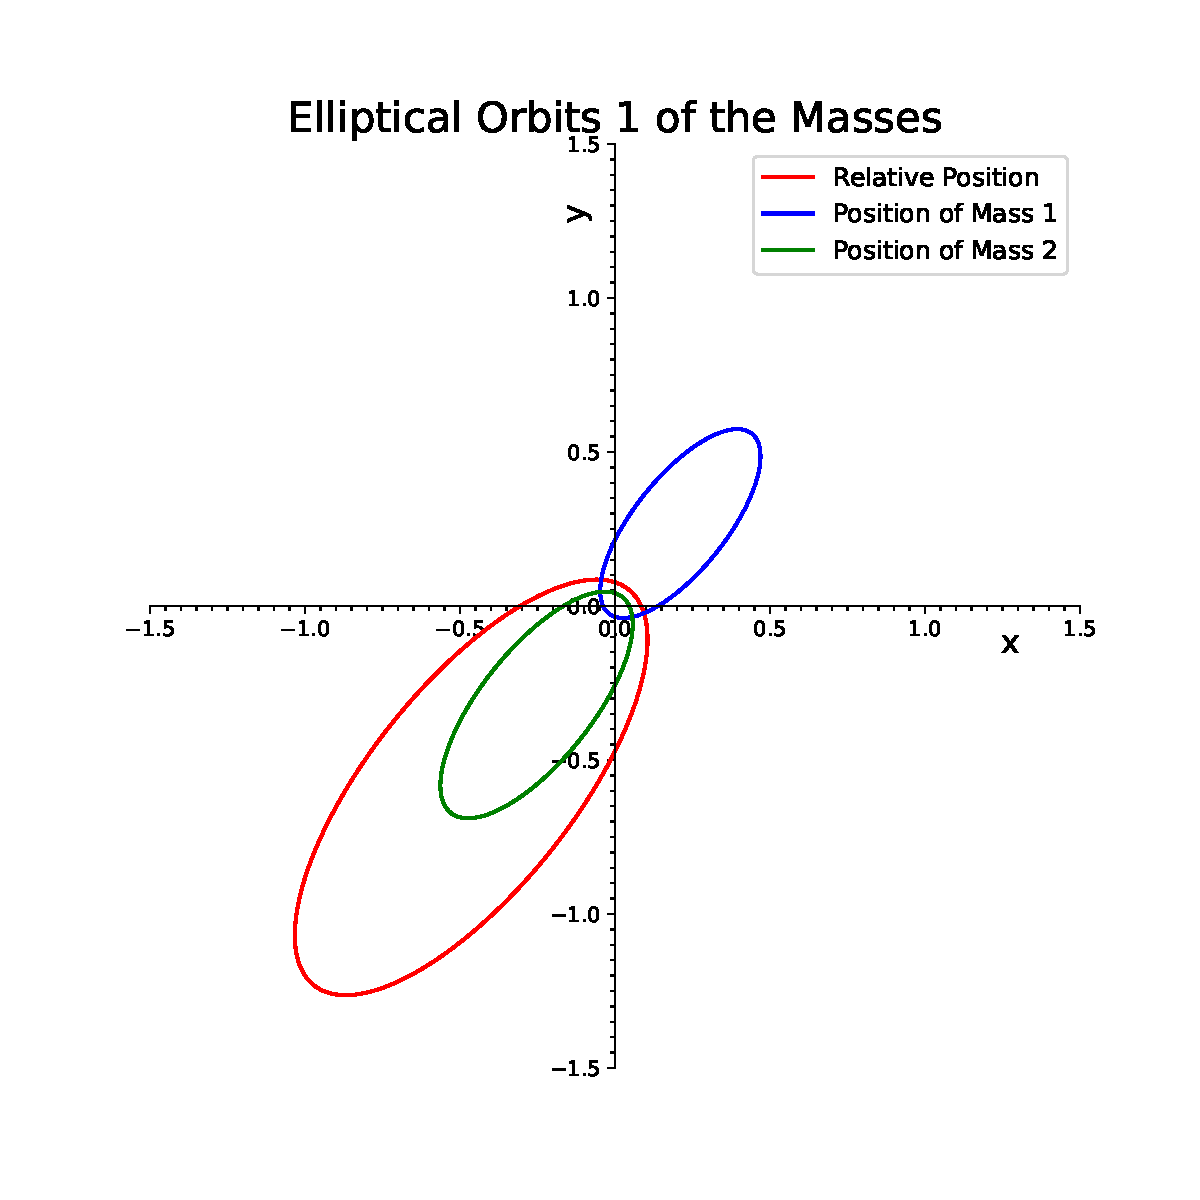
\includegraphics[width=7cm]{Elliptical Orbit 1.pdf}
    \caption{The image has shown an example of the elliptical orbits of the two masses. The orbits of the mass are indicated by the blue ellipse and the green ellipse. The red ellipse represents the relative position vector of the two masses.}\label{fig:Elliptical Orbit 1}
\end{SCfigure}

\begin{SCfigure}[25][t]
\caption{The image has shown another example of the elliptical orbits of the two masses, where the elliptical orbits could be seen as circular orbits. The orbits of the mass are indicated by the blue path and the green path. The red ellipse represents the relative position vector of the two masses.}\label{fig:Elliptical Orbit 2}
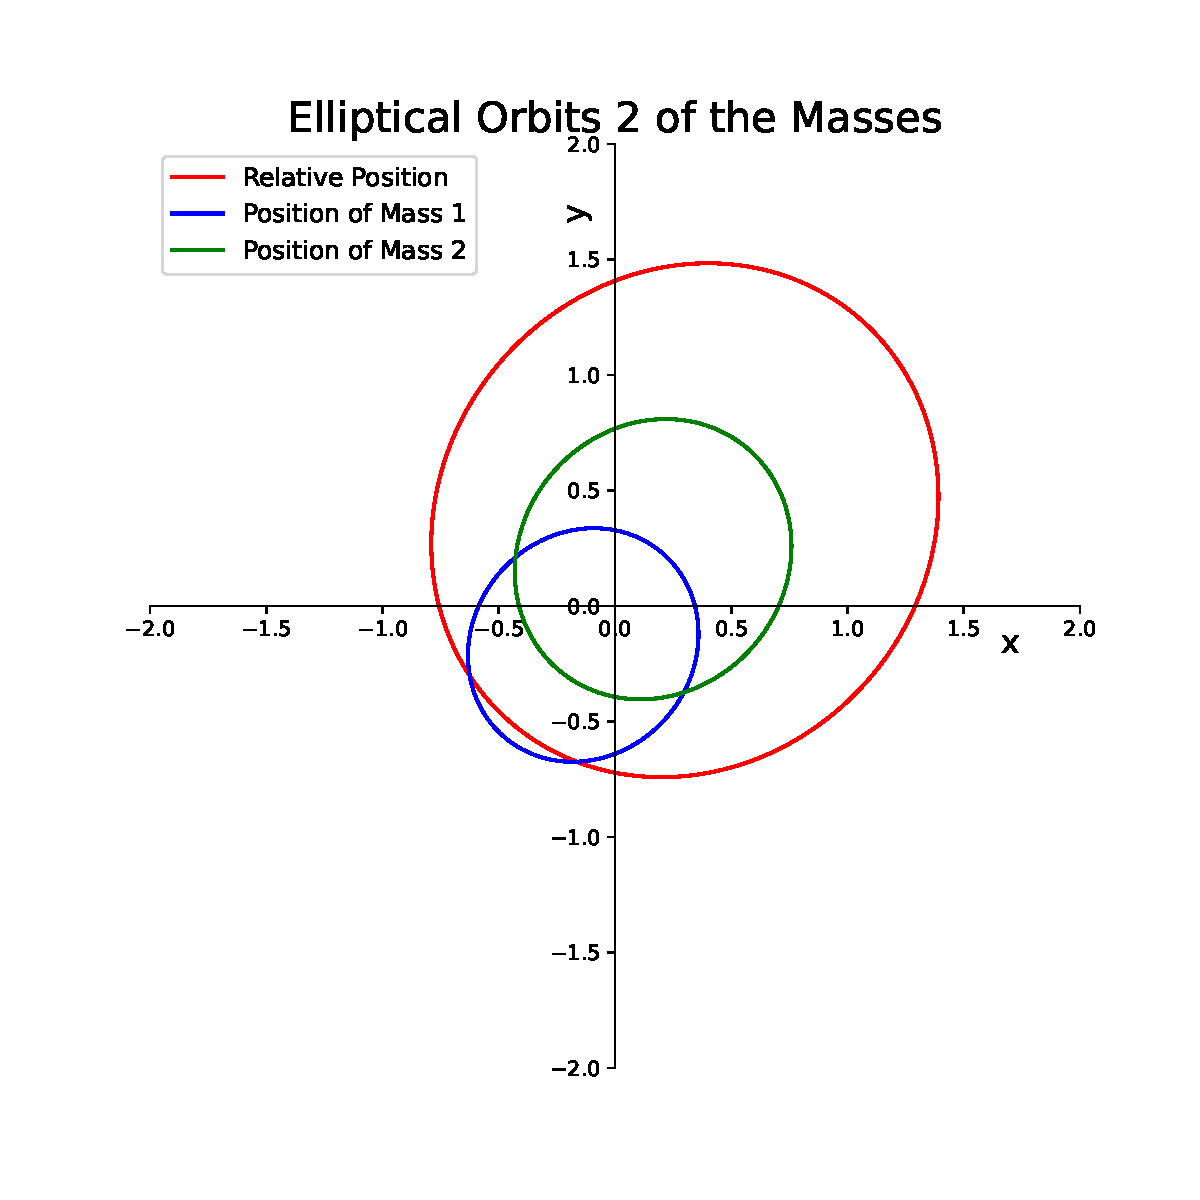
\includegraphics[width=7cm]{Elliptical Orbit 2.pdf}
\end{SCfigure}

\begin{SCfigure}[25][t]
\caption{This image has shown a hyperbolic trajectories of the two masses. The distance between of the two mass gets smaller first, and after a certain point, they start moving in the opposite directions and getting farther apart.}\label{fig:Hyperbolic Paths}
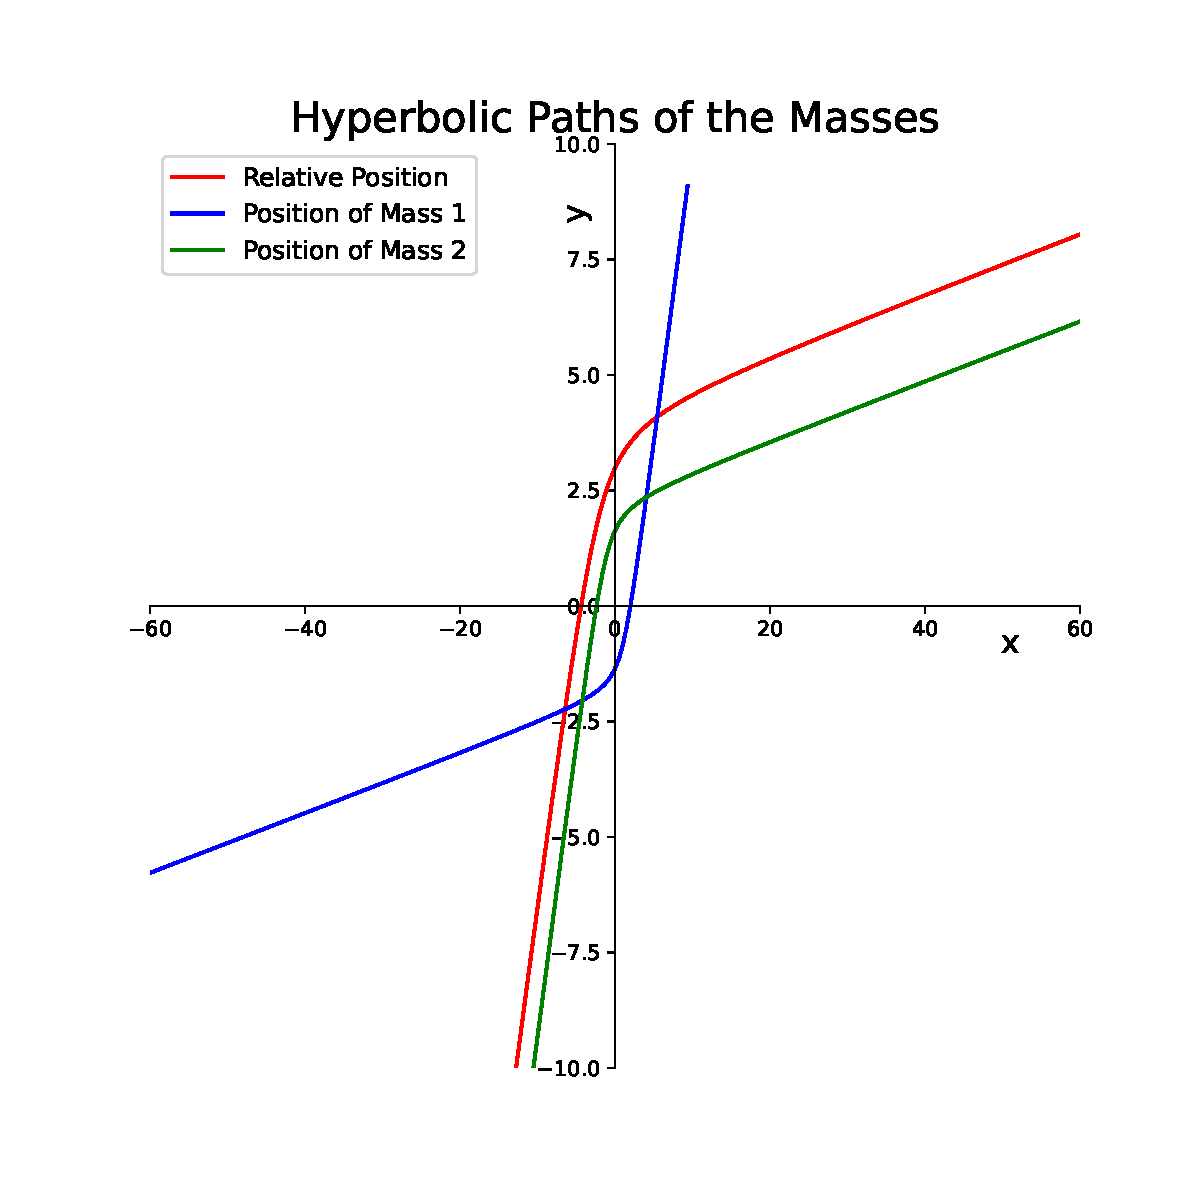
\includegraphics[width=7cm]{Hyperbolic Paths.pdf}
\end{SCfigure}

\newpage

\begin{figure}
    \centering
    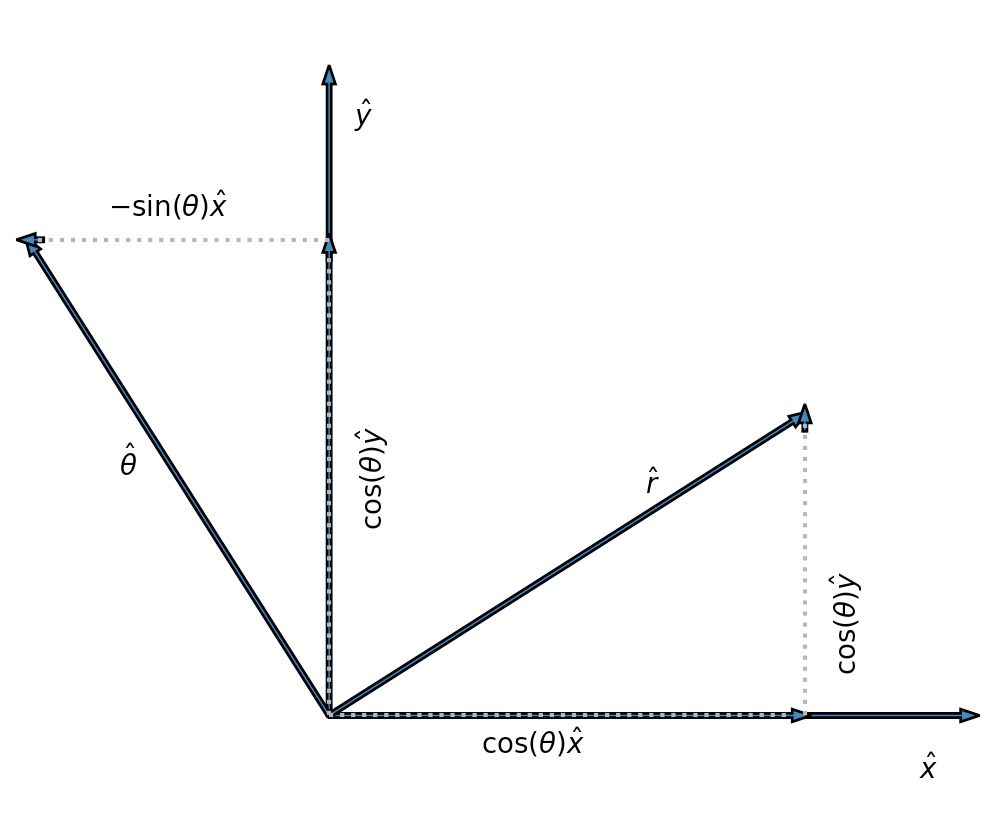
\includegraphics[width=0.5\textwidth]{Polar - Cartesian.png}
    \caption{Polar Coordinate and Cartesian Coordinate System}
    \label{fig:Polar - Cartesian}
\end{figure}

\newpage

\subsubsection{Analytical Calculations}
To solve for the general solution of their motion, we transform to a polar coordinate system $\left(r,\theta\right)$ referred to an origin centred on the mass $m_1$ and an arbitrary reference line corresponding to $\theta = 0$. Note that even though the centre of mass of $m_1$ and $m_2$ could be moving in inertial space, the direction of the reference line remains fixed. We let $\hat{\mathbf{r}}$ and $\hat{\boldsymbol{\theta}}$ denote unit vectors along and perpendicular to the radius vector respectively, so it is easy to find that $\hat{\mathbf{r}}$ and $\hat{\boldsymbol{\theta}}$ are perpendicular to each other. The image (\ref{fig:Polar - Cartesian}) has given us a clear illustration:
\begin{align}
    & \hat{\mathbf{r}} = \cos(\theta)\hat{\mathbf{x}} + \sin(\theta)\hat{\mathbf{y}}
    \label{hat mathbf r}\\
    & \hat{\boldsymbol{\theta}} = -\sin(\theta)\hat{\mathbf{x}} + \cos(\theta)\hat{\mathbf{y}}
    \label{hat mathbf theta}
\end{align}
Therefore,
\begin{align}
    & \frac{d\hat{\mathbf{r}}}{dt}
    = -\sin(\theta) \frac{d\theta}{dt}\hat{\mathbf{x}} + \cos(\theta) \frac{d\theta}{dt}\hat{\mathbf{y}}
    = \dot{\theta}\hat{\boldsymbol{\theta}}
    \label{Derivative of unit r}\\
    & \frac{d\hat{\boldsymbol{\theta}}}{dt}
    = -\cos(\theta) \frac{d\theta}{dt}\hat{\mathbf{x}} + (-\sin(\theta) \frac{d\theta}{dt}\hat{\mathbf{y}})
    = -\dot{\theta}\hat{\mathbf{r}}
    \label{Derivative of unit theta}
\end{align}
Now, we are capable of calculating $\mathbf{r}$, $\dot{\mathbf{r}}$, and $\ddot{\mathbf{r}}$ in polar coordinates, which are the position, velocity and the acceleration vectors. 
First of all, it is easy to get the position vector:
\begin{equation}
    \mathbf{r} = r \hat{\mathbf{r}},
    \label{polar coordinate position}
\end{equation}
where $r$ is the magnitude of the radius vector and $\hat{\mathbf{r}}$ denotes the direction of the vector.
Find the derivative of $r$, we can get the velocity vector:
\begin{align}
    \dot{\mathbf{r}} 
    & = \frac{dr}{dt}\hat{\mathbf{r}} + r\frac{d\hat{\mathbf{r}}}{dt} \notag\\
    & = \dot{r}\hat{\mathbf{r}} + r\dot{\theta}\hat{\boldsymbol{\theta}}
    \label{dot r}
\end{align}
Furthermore, find the derivative of the velocity vector gives us:
\begin{align}
    \ddot{\mathbf{r}}
    & = \frac{d\dot{r}}{dt}\hat{\mathbf{r}} + \dot{r}\frac{d\hat{\mathbf{r}}}{dt} + \frac{dr}{dt}\dot{\theta}\hat{\boldsymbol{\theta}} + r\frac{d\dot{\theta}}{dt}\hat{\boldsymbol{\theta}} + r\dot{\theta}\frac{d\hat{\boldsymbol{\theta}}}{dt} \notag\\
    & = \ddot{r}\hat{\boldsymbol{r}} + \dot{r}\dot{\theta}\hat{\boldsymbol{\theta}} + \dot{r}\dot{\theta}\hat{\boldsymbol{\theta}} + r\ddot{\theta}\hat{\boldsymbol{\theta}} + r\dot{\theta}(-\dot{\theta}\hat{\boldsymbol{r}}) \notag\\
    & = (\ddot{r} - r\dot{\theta}^2)\hat{\boldsymbol{r}} + (2\dot{r}\dot{\theta} + r\ddot{\theta})\hat{\boldsymbol{\theta}}\\
    & = (\ddot{r} - r\dot{\theta}^2)\hat{\boldsymbol{r}} + \left[ \frac{1}{r}\frac{d}{dt}(r^2\dot{\theta}) \right] \hat{\boldsymbol{\theta}}
    \label{ddot r}
\end{align}

Substituting the expression for $\dot{\mathbf{r}}$ into equation (\ref{eq:r and dot r}) gives:
\begin{align}
    \mathbf{h}
    & = r\hat{\mathbf{r}} \times (\dot{r}\hat{\mathbf{r}} + r\dot{\theta}\hat{\boldsymbol{\theta}}) \notag\\
    & = r\hat{\mathbf{r}} \times \dot{r}\hat{\mathbf{r}} + r\hat{\mathbf{r}} \times r\dot{\theta}\hat{\boldsymbol{\theta}} \notag\\
    & = r^2\dot{\theta} (\hat{\boldsymbol{r}} \times \hat{\boldsymbol{\theta}}).
\end{align}
Therefore,
\begin{equation}
    h = \left| \mathbf{h} \right| = r^2\dot{\theta}
    \label{eq:h=r2 dot theta}
\end{equation}

\begin{figure}[h]
    \centering
    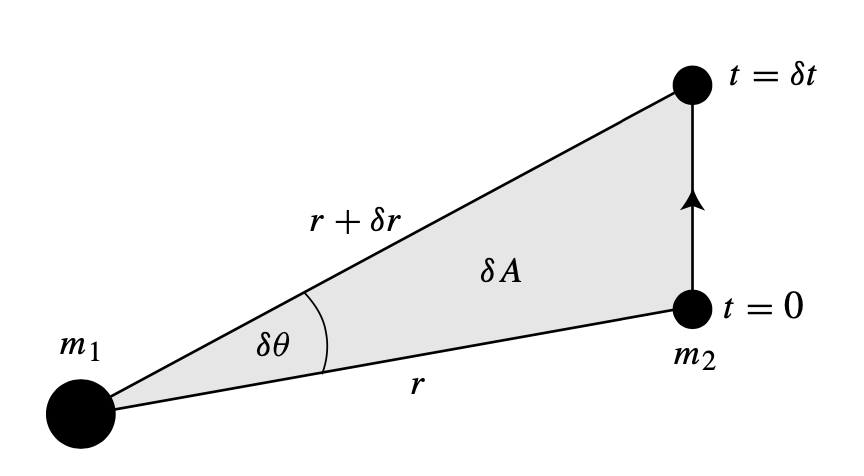
\includegraphics{area swiped.png}
    \caption{The area $\delta A$ swept out in a time $\delta t$ as a position vector moves through an angle $\delta \theta$.}
    \label{fig:area swiped}
\end{figure}

Consider the motion of the mass $m_2$ during a time interval $\delta t$ (see Fig. \ref{fig:area swiped}). At time t = 0 it has polar coordinates $(r, \theta)$, while at time $t + \delta t$ its polar coordinates have changed to $(r + \delta r, \theta + \delta \theta)$. The area, $\delta A$, swept out by the radius vector in time $\delta t$ is:
\begin{equation}
    \delta A \approx \frac{1}{2}r(r+\delta r)\sin(\delta \theta) \approx \frac{1}{2} r^2 \delta \theta.
\end{equation}
Therefore, by dividing each side by $\delta t$ and taking the limit as $\delta t \rightarrow 0$ we have:
\begin{equation}
    \frac{dA}{dt} = \frac{1}{2}r^2\frac{d\theta}{dt} = \frac{1}{2}h.
    \label{dA/dt = 1/2h}
\end{equation}
Since $h$ is a constant, this implies that equal areas are swept out in equal times and hence the above equation (\ref{dA/dt = 1/2h}) is the mathematical form of Kepler’s second law of planetary motion (\ref{Kepler Second Law}). Note that this does not require an inverse square law of force, but only that the force is directed along the line joining the two masses.

\subsection{Orbital Position and Velocity}
We obtain a scalar equation for the relative motion by substituting the expression for $\mathbf{\ddot{r}}$ from equation (\ref{ddot r}) into equation (\ref{eq:equation of relative motion}); comparing the $\hat{\mathbf{r}}$ components gives:
\begin{align}
    (\ddot{r} - r\dot{\theta}^2)\hat{\boldsymbol{r}} + \left[ \frac{1}{r}\frac{d}{dt}(r^2\dot{\theta}) \right] \hat{\boldsymbol{\theta}} + G(m_{2}+m_{1})\frac{r\hat{\mathbf{r}}}{r^3} & = 0 \notag\\
    \left[ (\ddot{r} - r\dot{\theta}^2) + G(m_{2}+m_{1})\frac{r}{r^3} \right] \hat{\mathbf{r}} + \left[ \frac{1}{r}\frac{d}{dt}(r^2\dot{\theta}) \right] \hat{\boldsymbol{\theta}} & = 0,
\end{align}
since we have already knew that $\hat{\boldsymbol{r}}$ and $\hat{\boldsymbol{\theta}}$ are two orthogonal unit vectors, hence:
\begin{equation}
    \left[ (\ddot{r} - r\dot{\theta}^2) + G(m_{2}+m_{1})\frac{r}{r^3} \right] = 0 ~~~~~or~~~~~ \left[ \frac{1}{r}\frac{d}{dt}(r^2\dot{\theta}) \right] = 0
\end{equation}
we also know $h = r^2\dot{\theta} = constant$ from equation (\ref{eq:h=r2 dot theta}), which means $\frac{d}{dt}(r^2\dot{\theta}) = 0$. This implies us:
\begin{equation}
    \ddot{r} - r\dot{\theta}^2 = -\frac{G(m_{2}+m_{1})}{r^2}
    \label{relative motion equation 2}
\end{equation}
In order to solve this equation and find $r$ as a function of $\theta$ we need to make the substitution $u = 1/r$ and to eliminate the time by making use of the constant $h = r^2 \dot{\theta}$. By differentiating $r$ with respect to time, we can get:

\begin{minipage}[t]{0.45\textwidth}
    \begin{align*}
        \frac{dr}{dt}
        & = \left( \frac{dr}{du} \right) \left( \frac{du}{d\theta} \right) \left( \frac{d\theta}{dt} \right) \notag\\
        & = -\frac{1}{u^2} \left( \frac{du}{d\theta} \right) \dot{\theta} \notag\\
        & = -h \left( \frac{du}{d\theta} \right), \notag\\
    \end{align*} \notag
\end{minipage} \notag
\begin{minipage}[t]{0.45\textwidth}
    \begin{align}
        \frac{d^2r}{dt^2} 
        & = \frac{d}{dt}\left( \frac{dr}{dt} \right) \notag\\
        & = \frac{d\theta}{dt} \left( \frac{d}{d\theta} \right) \left[ \left( \frac{d\theta}{dt} \right) \left( \frac{du}{d\theta} \right) \left( \frac{dr}{du} \right) \right] \notag\\
        & = \dot{\theta} \left( \frac{d}{d\theta} \right) \left[ \dot{\theta} \left( \frac{du}{d\theta} \right) (-r^2) \right] \notag\\
        & = -\dot{\theta} \frac{d}{d\theta} \left( h \frac{du}{d\theta} \right) \notag\\
        & = -\dot{\theta} h \frac{d^2u}{d\theta^2} \notag\\
        & = -h^2u^2 \frac{d^2u}{d\theta^2},
        \label{d2r/dtheta2}
    \end{align}
\end{minipage}

and therefore, substituting equation (\ref{d2r/dtheta2}) into equation (\ref{relative motion equation 2}):
\begin{align}
    -h^2u^2 \left( \frac{d^2u}{d\theta^2} \right) - r\dot{\theta}^2 & = -\frac{G(m_{2}+m_{1})}{r^2} \notag\\
    \frac{d^2u}{d\theta^2} + \frac{r\dot{\theta}^2}{h^2u^2} & = \frac{G(m_{2}+m_{1})}{r^2h^2u^2} \notag\\
    \frac{d^2u}{d\theta^2} + u & = \frac{G(m_{2}+m_{1})}{h^2} 
    \label{non-homogeneous differential eq}
    \tag{44}
\end{align}

In order to solve the above nonhomogeneous differential equation (\ref{non-homogeneous differential eq}), we need to solve the homogeneous differential equation first:
\begin{equation}
    \frac{d^2u}{d\theta^2} + u = 0.
    \tag{45}
\end{equation}
From the above homogeneous differential equation, we are able to obtain the characteristic equation:
\begin{equation}
    x^2 + 1 = 0
    \tag{46}
\end{equation}
Easy to find the solutions for the characteristic equation:
\begin{equation}
    x_1 = i ~~~~~~~or~~~~~~~ x_2 = -i
    \tag{47}
\end{equation}
therefore,
\begin{align}
    u(\theta)
    & = C_1e^{i\theta} + C_2e^{-i\theta} \notag\\
    & = C_1 \cos(\theta) + C_1 i \sin(\theta) + C_2 \cos(\theta) - C_2 i \sin(\theta) \notag\\
    & = (C_1 + C_2) \cos(\theta) + (C_1 - C_2) i \sin(\theta),
\end{align}
where $C_1$ and $C_2$ are two constants.
We also know that $u = 1/r$ where $r$ is a real value, hence $u$ must be a real value as well, so:
\begin{equation}
    u(\theta) = R_1 \cos(\theta) + R_2 \sin(\theta),
    \tag{48}
\end{equation}
where $R_1$ and $R_2$ are two real numbers.

So the solution for the nonhomogeneous differential equation (\ref{non-homogeneous differential eq}) is:
\begin{equation}
    u(\theta) = R_1 \cos(\theta) + R_2 \sin(\theta) + \frac{G(m_{2}+m_{1})}{h^2},
    \tag{49}
\end{equation}
using the auxiliary angle formula solve for $u(\theta)$:
\begin{align}
    u(\theta) 
    & = \sqrt{{R_1}^2 + {R_2}^2} \cos(\theta - \overline{\omega}) + \frac{G(m_{2}+m_{1})}{h^2} \notag\\
    & = \frac{G(m_{2}+m_{1})}{h^2} \left[ \frac{\sqrt{{R_1}^2 + {R_2}^2} h^2}{G(m_{2}+m_{1})} \cos(\theta - \overline{\omega}) + 1 \right] \notag\\
    & = \frac{G(m_{2}+m_{1})}{h^2} \left[ e \cos(\theta - \overline{\omega}) + 1 \right],
    \tag{50}
\end{align}
where $e$ (an amplitude) and $\overline{\omega}$ (a phase) are two constants of integration. Substituting back for $r$ we have:
\begin{equation}
    r = \frac{p}{e \cos(\theta - \overline{\omega}) + 1},
    \tag{51}
\end{equation}
which is the general equation of a conic in polar coordinates where $e$ is the eccentricity and $p$ is the semilatus rectum given by
\begin{equation}
    p = h^2 / G(m_{2}+m_{1}).
    \label{p and h relation}
    \tag{52}
\end{equation}

In order to gain a better understanding about the conic sections, we give two real quantities $a > 0$ and $e > 0$ with $e \ne 1$ since it would be a circle as $e=1$, we further define the auxiliary quantities $c = a \cdot e$ and $d = a/e$.
Define the $\textsl{focus}$ as the point $F(c,0)$ and the $\textsl{directrix}$ as the vertical line $D$ with equation $x = d$ .

Consider the set $C = C(a,e)$ defined as the set of all points $P(x,y)$ in the plane which satisfy the condition
\begin{equation}
    PF = e ( PD ),
    \tag{53}
\end{equation}
so the points of $C(a,e)$ are described by
\begin{align}
    PF^2 & = e^2 (PD)^2 \notag\\
    (x - c)^2 + (y - 0)^2 & = e^2 (x - d)^2 \notag\\
    (1 - e^2)x^2 + y^2 + 2(de^2 - c)x & = e^2 d^2 - c^2. 
    \tag{54}
\end{align}
Since $de^2 = c$ and $de = a$ we find that the points of $C(a,e)$ are characterized by the equation:
\begin{equation}
    (1 - e^2)x^2 + y^2 = a^2 - c^2 
    \tag{55}
\end{equation}
If $0<e<1$, we would obtain the standard equation of an ellipse:
\begin{equation}
    \frac{x^2}{a^2} + \frac{y^2}{a^2 - c^2} = 1,
    \tag{56}
\end{equation}
On the other hand, if $1<e$, we can obtain the standard equation of a hyperbola:
\begin{equation}
    \frac{x^2}{a^2} - \frac{y^2}{a^2 - c^2} = 1,
    \tag{57}
\end{equation}
Recall that the parabola was defined in terms of a focus $F(p,0)$ where $p > 0$ and the directrix $D$ with equation $x = -p$ in terms of the condition:
\begin{equation}
    PF = 1 ( PD ).
    \tag{58}
\end{equation}
In conclusion, the four possible conics in our two-body situation are (\cite{CURTIS2014xi}):
\begin{align}
    & circle: && e = 0, && p=a; \notag\\
    & ellipse: && 0 < e < 1, && p=a(1-e^2); \notag\\
    & parabola: && e = 1, && p = 2q; \notag\\
    & hyperbola: && e > 1, && p = a(e^2-1), \notag
\end{align}
where the constant $a$ is the semi-major axis of the conic. In the special case of the parabola $p$ is defined in terms of $q$, the distance to the central mass at closest approach. The conic section curves derive their name from the curves formed by the intersection of various planes with the surface of a cone (see figure \ref{fig:conic sections}).

\begin{SCfigure}
    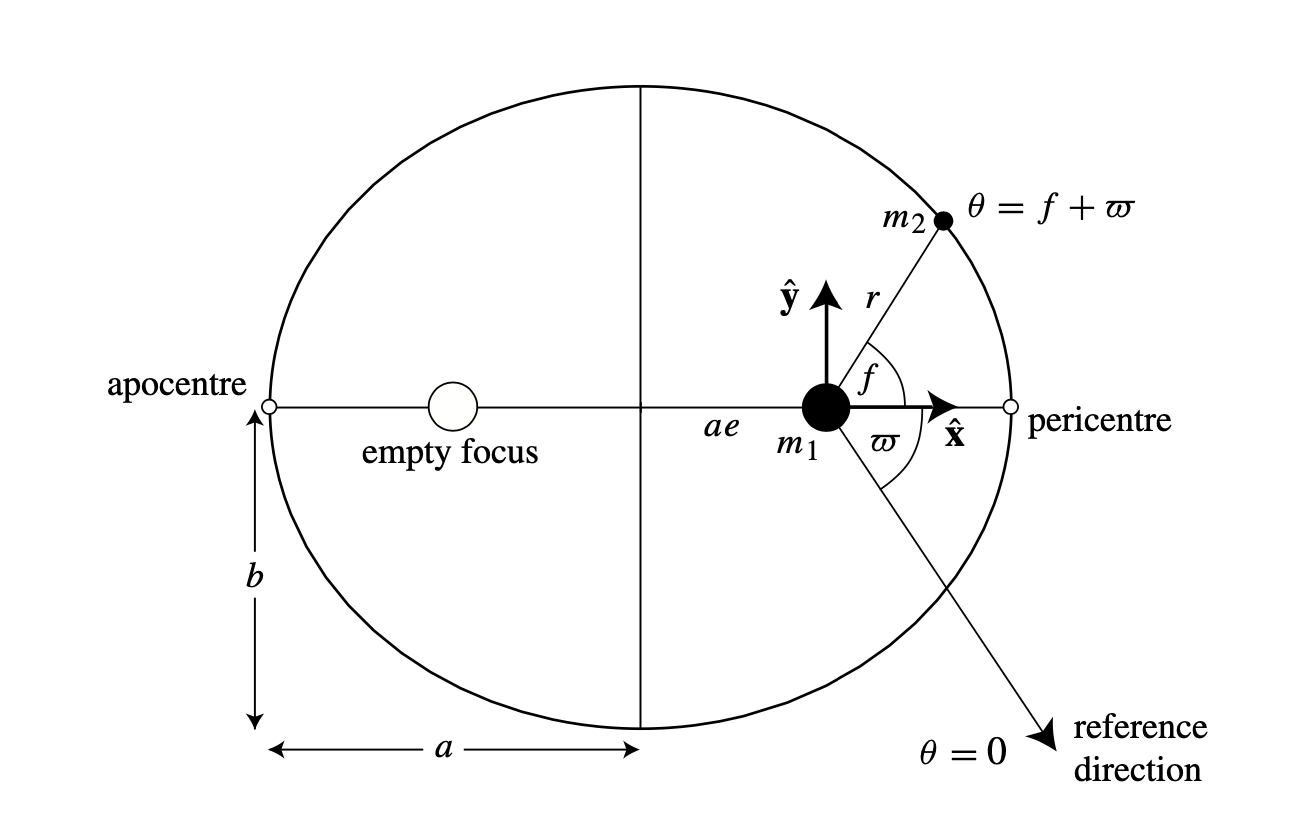
\includegraphics[width=0.7\textwidth]{Ellipse.png}
    \caption{The geometry of the ellipse of semi-major axis $a$, semi-minor axis $b$, eccentricity $e$, and longitude of pericentre $\overline{\omega}$ .}
    \label{fig:ellipse}
\end{SCfigure}

We focus on the elliptical motion. In this case $p = a(1-e^2)$ and the quantities $a$ and $e$ are related by
\begin{equation}
    b^2 = a^2 (1-e^2),
    \label{b a e relation}
    \tag{59}
\end{equation}
where $b$ is the $\textit{semi-minor axis}$ of the ellipse (see figure \ref{fig:ellipse}); we also have that
\begin{equation}
    r = \frac{a(1 - e^2)}{1 + e \cos(\theta - \overline{\omega})},
    \label{elliptical r}
    \tag{60}
\end{equation}
where the angle $\theta$ is called the $true ~longitude$. We could easily find that the minimum and maximum values of the orbital radius are $r_q = a(1-e)$ and $r_a = a(1+e)$, which occur when $\theta = \overline{\omega}$ and $\theta = \overline{\omega} + \pi$ respectively. These points in the orbits are called the $pericentre$ and the $apocentre$ respectively. Note that the distance of either focus from the centre of the ellipse is $ae$.

The angle $\overline{\omega}$ (pronounced “curly pi”) is called the $longitude ~of ~pericentre$. Although this is a constant for the two-body problem, it can vary with time when additional perturbations are introduced. We now introduce the angle $f = \theta - \overline{\omega}$ (see figure \ref{fig:ellipse}), which is called the $true ~anomaly$. Since $\overline{\omega}$ is constant the path is closed and the angular position is described by $f$ or $\theta$, which are $2\pi$-periodic variables. Hence equation (\ref{elliptical r}) can be written as
\begin{equation}
    r = \frac{a(1 - e^2)}{1 + e \cos(f)},
    \tag{61}
\end{equation}
Using a Cartesian Coordinate System centred on the central mass with the x axis pointing towards the pericentre (figure \ref{fig:ellipse}), then the components of the position vector are
\begin{equation}
    x = r \cos(f) ~~~~~~~~and~~~~~~~~ y = r \sin(f)
    \tag{62}
\end{equation}

In one orbital period $T$ the area swept out by a radius vector is simply the area $A = \pi ab$ enclosed by the ellipse. From equation (\ref{dA/dt = 1/2h}) this area has to equal to $hT/2$, and from equation (\ref{p and h relation}), introducing $\mu = G(m_2 + m_1)$, we obtain
\begin{align}
    \left( \frac{hT}{2} \right)^2 = (\pi ab)^2 \notag\\
    \frac{\mu a(1-e^2) T^2}{4} = \pi^2 a^2 b^2, \notag\\
\end{align}
and from equation (\ref{b a e relation}), we can further know that
\begin{align}
    \frac{\mu b^2 T^2}{4a} = \pi^2 a^2 b^2,
    \tag{63}
\end{align}
therefore
\begin{equation}
    T^2 = \frac{4 \pi^2}{\mu} a^3,
    \label{T and a relation}
    \tag{64}
\end{equation}
which corresponds to Kepler's third law of planetary motion (Sect. \ref{Kepler's Laws}). Note that the period of the orbit is independent of $e$ and is a function of $\mu$ and $a$ only.

Consider the case of two objects of mass $m$ and $m'$, orbiting a central object of mass $m_c$. Let the orbiting objects have semi-major axes $a$ and $a'$ and orbital periods $T$ and $T'$ where we know  from equation (\ref{T and a relation})
\begin{align}
    T^2 = \frac{4 \pi^2}{\mu} a^3 ~~~~~~and~~~~~~ T'^2 = \frac{4 \pi^2}{\mu'} a'^3,
    \tag{65}
\end{align}
then we could get
\begin{align}
    \frac{T'^2}{T^2} = \frac{\frac{4 \pi^2}{\mu'} a'^3}{\frac{4 \pi^2}{\mu} a^3}
    \tag{66}
    \label{two orbiting objects relation}
\end{align}
Simplify equation (\ref{two orbiting objects relation})
\begin{equation}
    \frac{m_c + m}{m_c + m'} = \left( \frac{a}{a'} \right)^3 \left( \frac{T'}{T} \right)^2
    \tag{67}
\end{equation}
In the case of planets orbiting the Sun we have $m, m' \ll m_c$ and hence $(a/a')^3 \approx (T/T')^2$. Therefore, if $a$ and $T$ denote the values of the semi-major axis and the period of the Earth’s orbit and the unit of length is taken to be the $\textit{astronomical unit} ~AU$ (1 $AU$ is the approximate semi-major axis of the Earth’s orbit) and the unit of time is taken to be the year (the approximate period of the Earth’s orbit), we have $T' \approx a'^{3/2}$.

If any solar system object (e.g., an asteroid or a comet) has a small natural or artificial satellite, then observations of the distance and period of the satellite can be used with Kepler’s third law to derive an estimate of the mass of the object.





\section{Three-Body Problem} 

Two’s company, three’s a crowd.

\subsection{Introduction of Three Body Problem}

In the previous chapter, we showed how the problem of the motion of two masses moving under their mutual gravitational attraction can be solved analytically. We will now extend our analysis to consider the gravitational interaction of three bodies. The three body problem is a special case in the n-body problems. We are now determining the motion of three celestial bodies moving under no influence other than that of their mutual gravitation. Unlike two-body problems, no general closed-form solution exists, as the resulting dynamical system is chaotic for most initial conditions, and numerical methods are generally required. The elusiveness of it has obsessed mathematicians and physicists for centuries. The most classical example for the three body problem is the system made up of the sun, the earth and the moon, while the motion of the earth and the moon disturbed by the action of the sun. 

In this chapter, we will explore some special cases in the three body problem, and dig into the three body problem, try to find the numerical solutions for it


\subsection{Restricted Three Body Problem}

In this section, we give several restrictions to our three bodies in the three body problem. For the three objects in our system, we assume one of the objects having a much greater mass comparing to the other two, while another one object having a much smaller mass. Reasonably, the object with the medium mass would orbit around the heaviest object in a circular path, where the gravitational force exerted by the lightest object on it would be disregarded, while the object with the smallest mass would experience both gravitational forces exerted by the two other objects. 

Using the code shown in the file $\textit{Restricted Three Body Problem 2D}$ (appendix \ref{Appendix A}) we simulate the system of a three body problem. Since we have assumed the sun (object with the largest mass) is motionless at the centre of the system, and the path of the planet (object with the medium mass), which can be described as a circle, $(x,y) = (\cos(t),\sin(t))$, so we only need to solve for the orbit of the asteroid (object with the smallest mass).

We have already know the total force acting on the asteroid are the gravitational forces:
\begin{align}
    F_{total} 
    & = m_{asteroid} \cdot a \notag \\
    & = \frac{G \left( m_{asteroid} \right) \left( m_{sun} \right)}{r_{SA}^2} \left( \frac{\mathbf{r}_{SA}}{\left| \mathbf{r}_{SA} \right|} \right) + \frac{G \left( m_{asteroid} \right) \left( m_{planet} \right)}{r_{PA}^2} \left( \frac{\mathbf{r}_{PA}}{\left| \mathbf{r}_{PA} \right|} \right) \tag{68},
\end{align}
where $\mathbf{r}_{SA}$ denotes the vector between the sun and the asteroid pointing towards the asteroid, and $\mathbf{r}_{PA}$ denotes the vector between the planet and the asteroid pointing towards the asteroid. Hence,
\begin{align*}
    a 
    & = \frac{d^2 r}{d t^2} \\
    & = \frac{G \left( m_{sun} \right) \left( \mathbf{r}_{SA} \right)}{r_{SA}^3} + \frac{G \left( m_{planet} \right) \left( \mathbf{r}_{PA} \right)}{r_{PA}^3} \tag{69}.
\end{align*}
For convenience, we let the value for $G$ to be 1, the mass of the sun to be 1, and the mass for the planet to be 0.01. Therefore,
\begin{align*}
    \frac{d^2 r}{d t^2} 
    & = \frac{\mathbf{r}_{SA}}{r_{SA}^3} + \frac{m_{planet} \left( \mathbf{r}_{PA} \right)}{r_{PA}^3} \\
    & = \frac{\mathbf{r}_{A} - \mathbf{r}_{S}}{(r_{A} - r_{S})^3} + \frac{m_{planet} (\mathbf{r}_{A} - \mathbf{r}_{P})}{(r_{A} - r_{P})^3} \tag{70}.
\end{align*}
After decomposing $\frac{d^2 r}{d t^2}$ into $x$ and $y$ components, we find the $x$ and $y$ values for different value of time, t. Hence, we are able to use the function $\textsl{odeint()}$ to help us solving the first order differential equations.



\begin{figure}[h]
    \centering % <-- added
\begin{subfigure}{0.4\textwidth}
  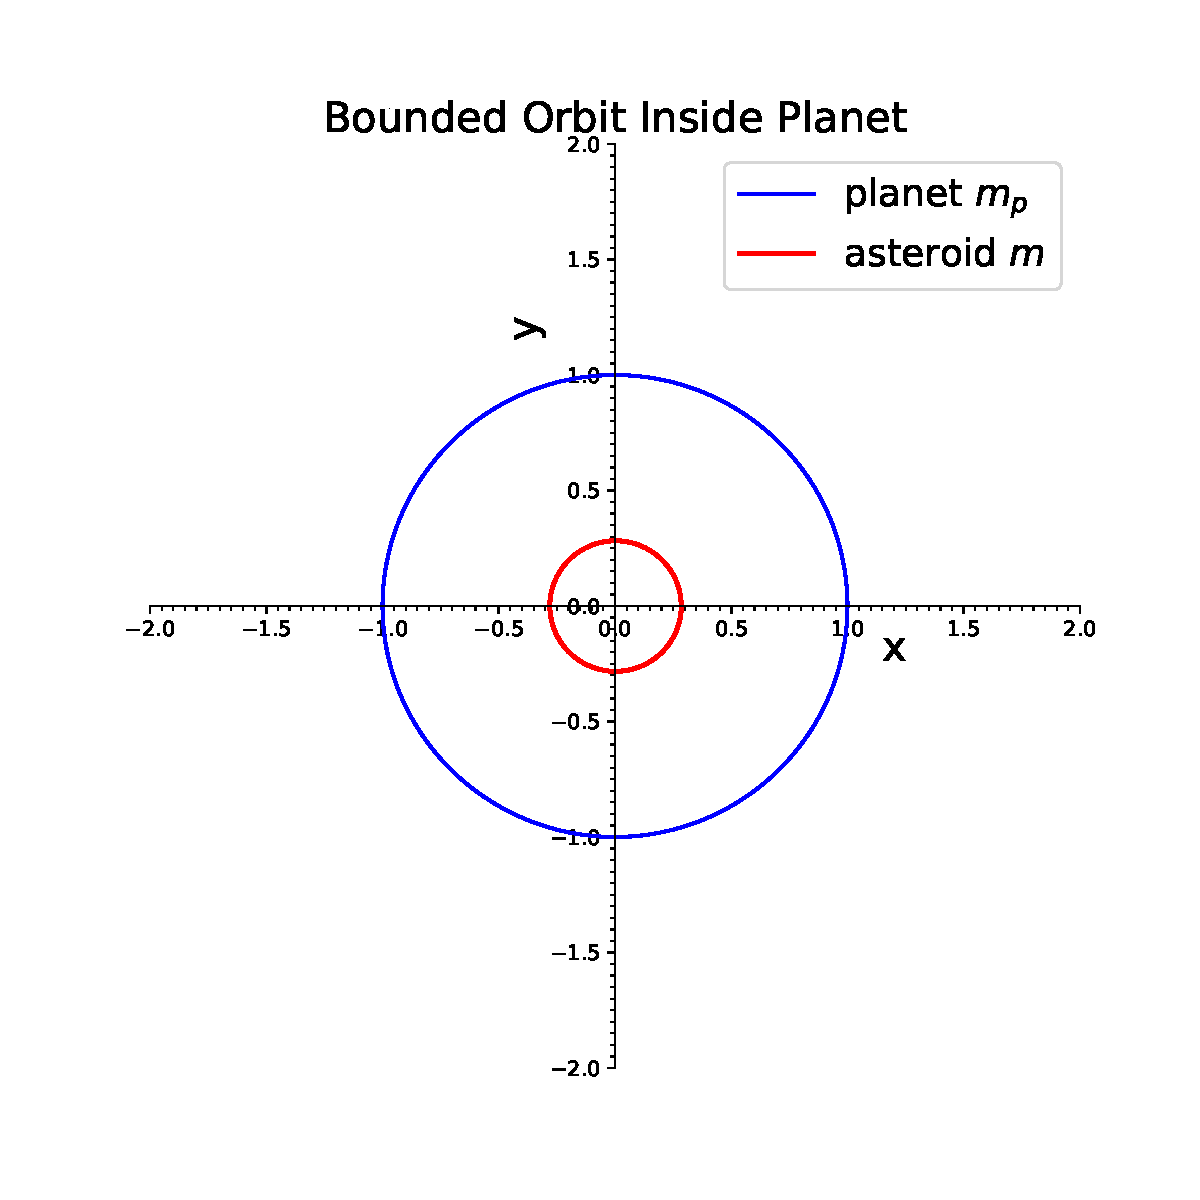
\includegraphics[width=\linewidth]{orbit1.pdf}
  \caption{the planet and the asteroid are moving on circular orbits, while the planet is orbiting outside the path of the asteroid. (The sun is at the centre with the mass much bigger than both the planet and the asteroid)}
  \label{fig:1}
\end{subfigure}\hfil % <-- added
\begin{subfigure}{0.4\textwidth}
  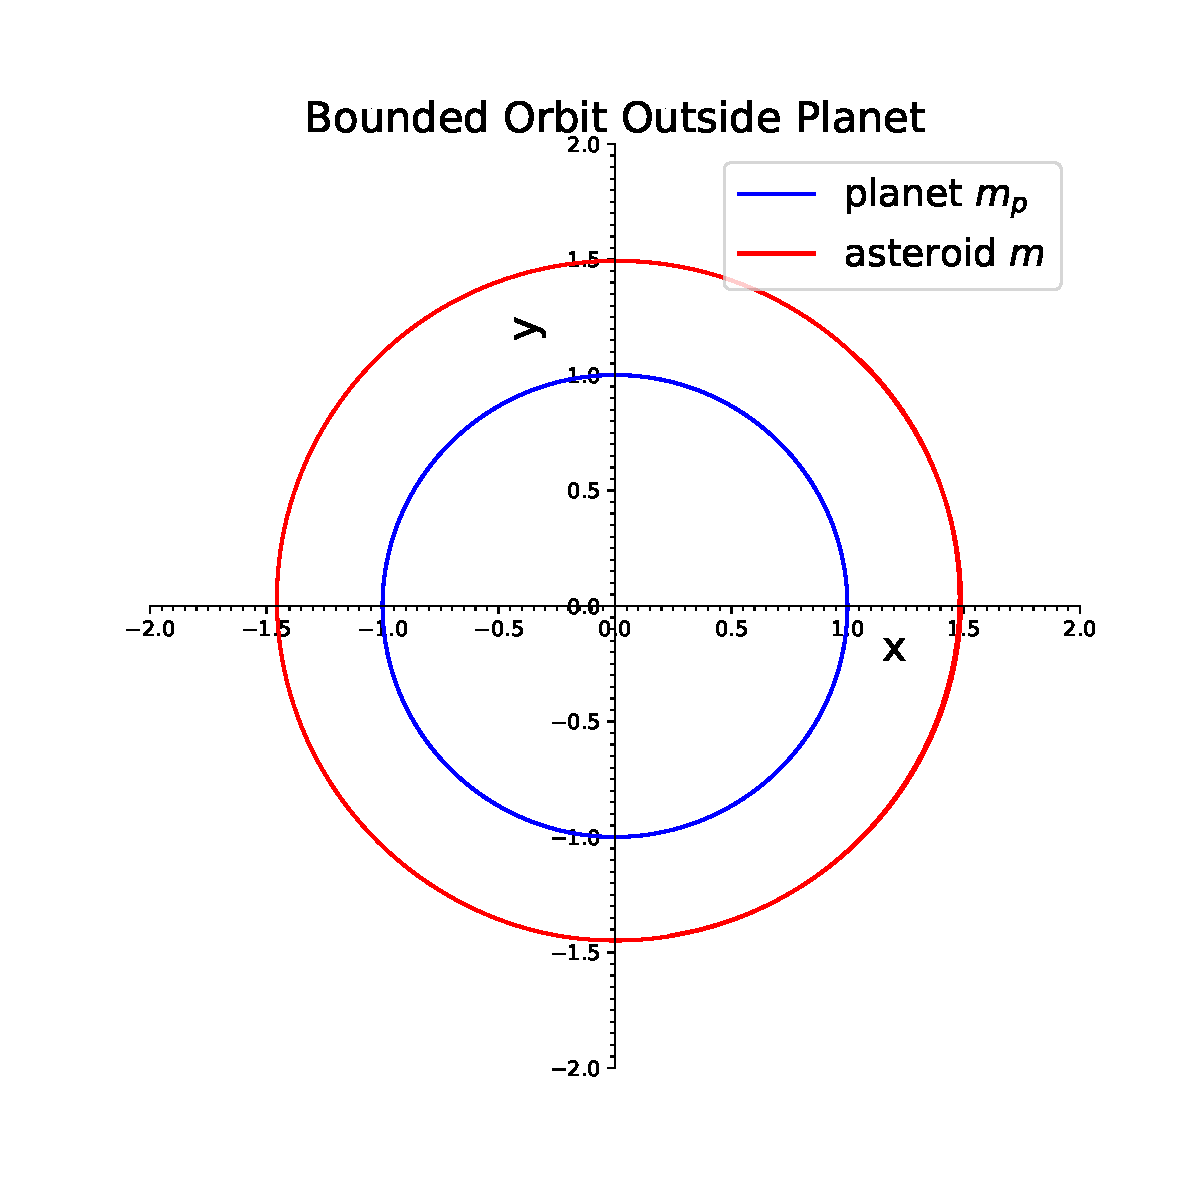
\includegraphics[width=\linewidth]{orbit2.pdf}
  \caption{the planet and the asteroid are moving on circular orbits, while the asteroid is orbiting outside the path of the planet. (The sun is at the centre with the mass much bigger than both the planet and the asteroid)}
  \label{fig:2}
\end{subfigure}\hfil % <-- added
\end{figure}

\begin{figure}[p]
    \centering % <-- added
\begin{subfigure}{0.4\textwidth}
  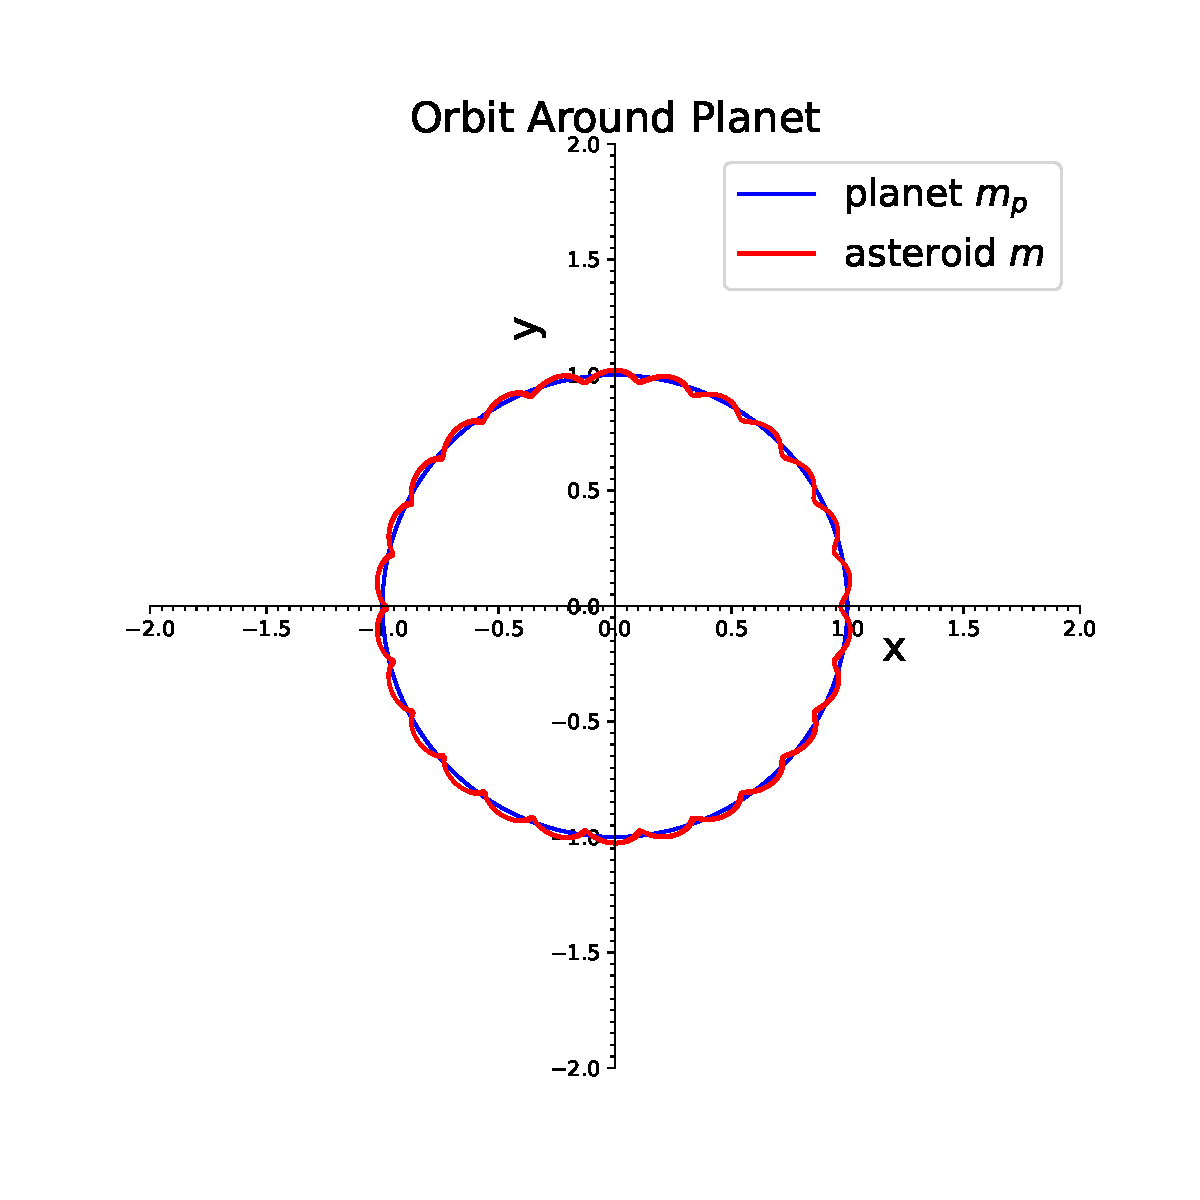
\includegraphics[width=\linewidth]{orbit4.pdf}
  \caption{the planet is orbiting the sun in a circular path, while the asteroid is surrounding the planet, orbiting the planet consistently (The sun is at the centre)}
  \label{fig:4}
\end{subfigure}\hfil % <-- added
\begin{subfigure}{0.4\textwidth}
  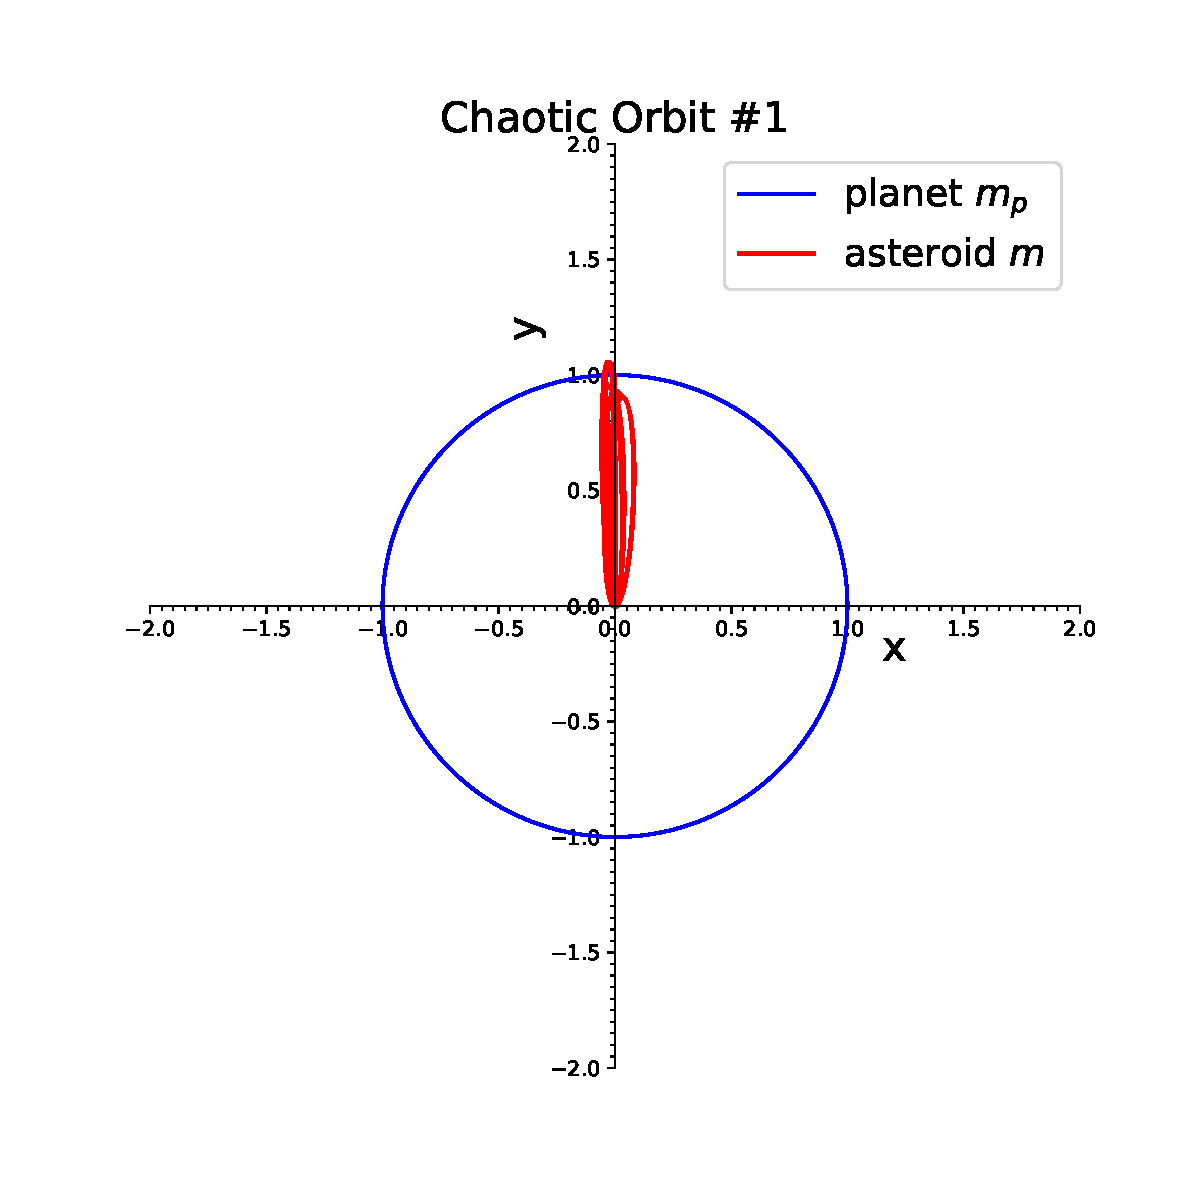
\includegraphics[width=\linewidth]{orbit5.pdf}
  \caption{the planet is orbiting the sun in a circular path, while the asteroid is moving between the orbit of the planet and the sun back and forth chaotically along the y-axis. (The sun is at the centre)}
  \label{fig:5}
\end{subfigure}\hfil % <-- added

\medskip
\begin{subfigure}{0.4\textwidth}
  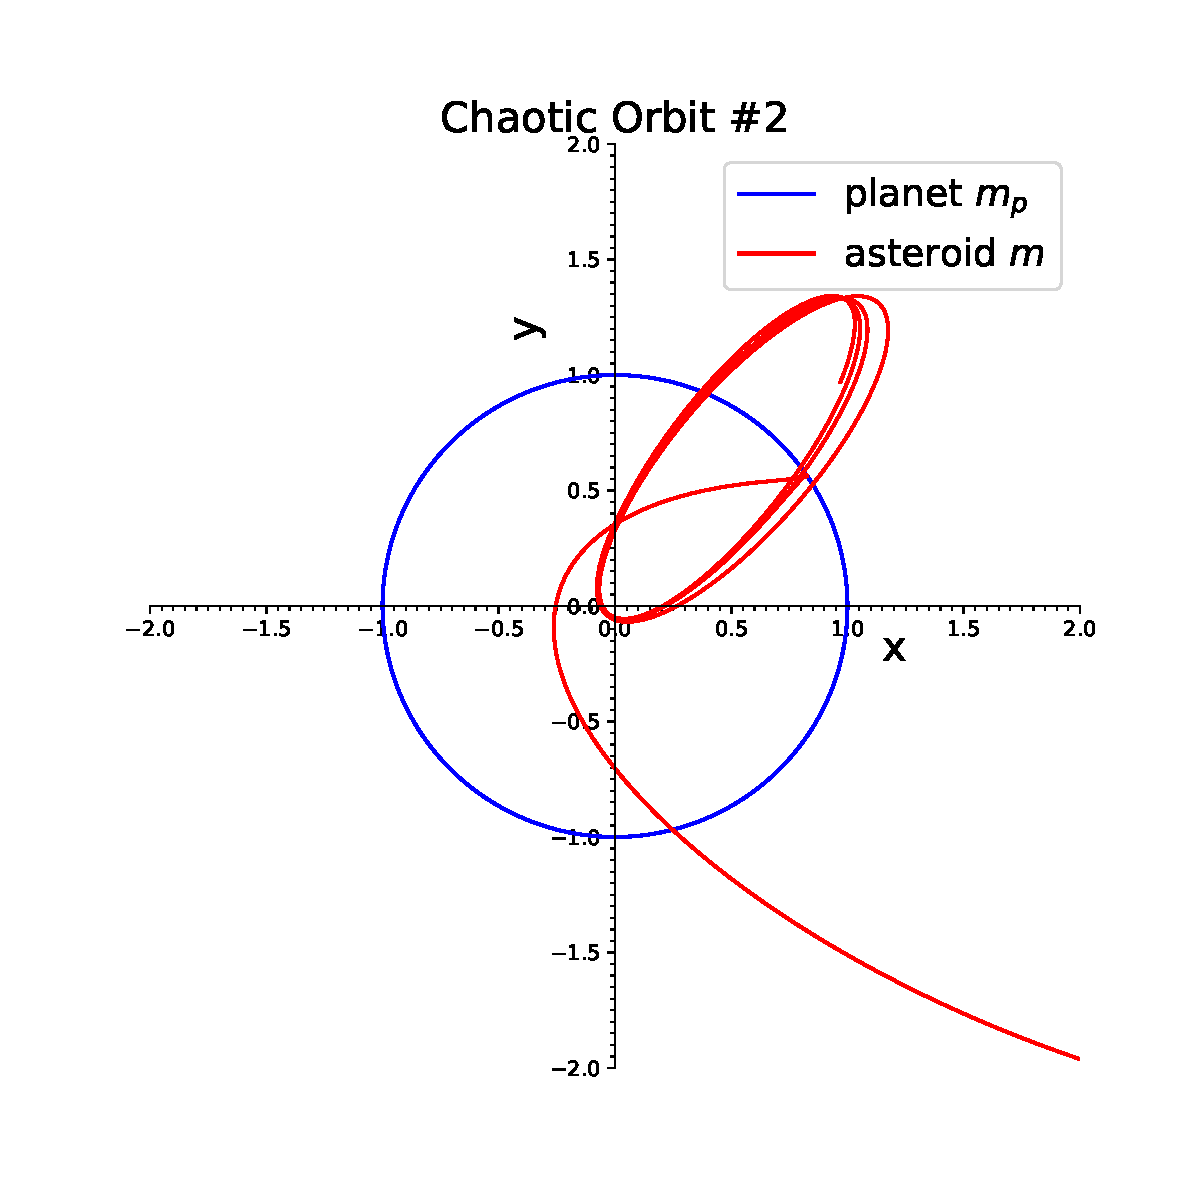
\includegraphics[width=\linewidth]{orbit6.pdf}
  \caption{the planet is orbiting the sun in circular path, while the asteroid is moving in an elliptical path in the first quadrant of the coordinate system at the beginning, and then leaving the system with an parabolic path. }
  \label{fig:4}
\end{subfigure}\hfil % <-- added
\begin{subfigure}{0.4\textwidth}
  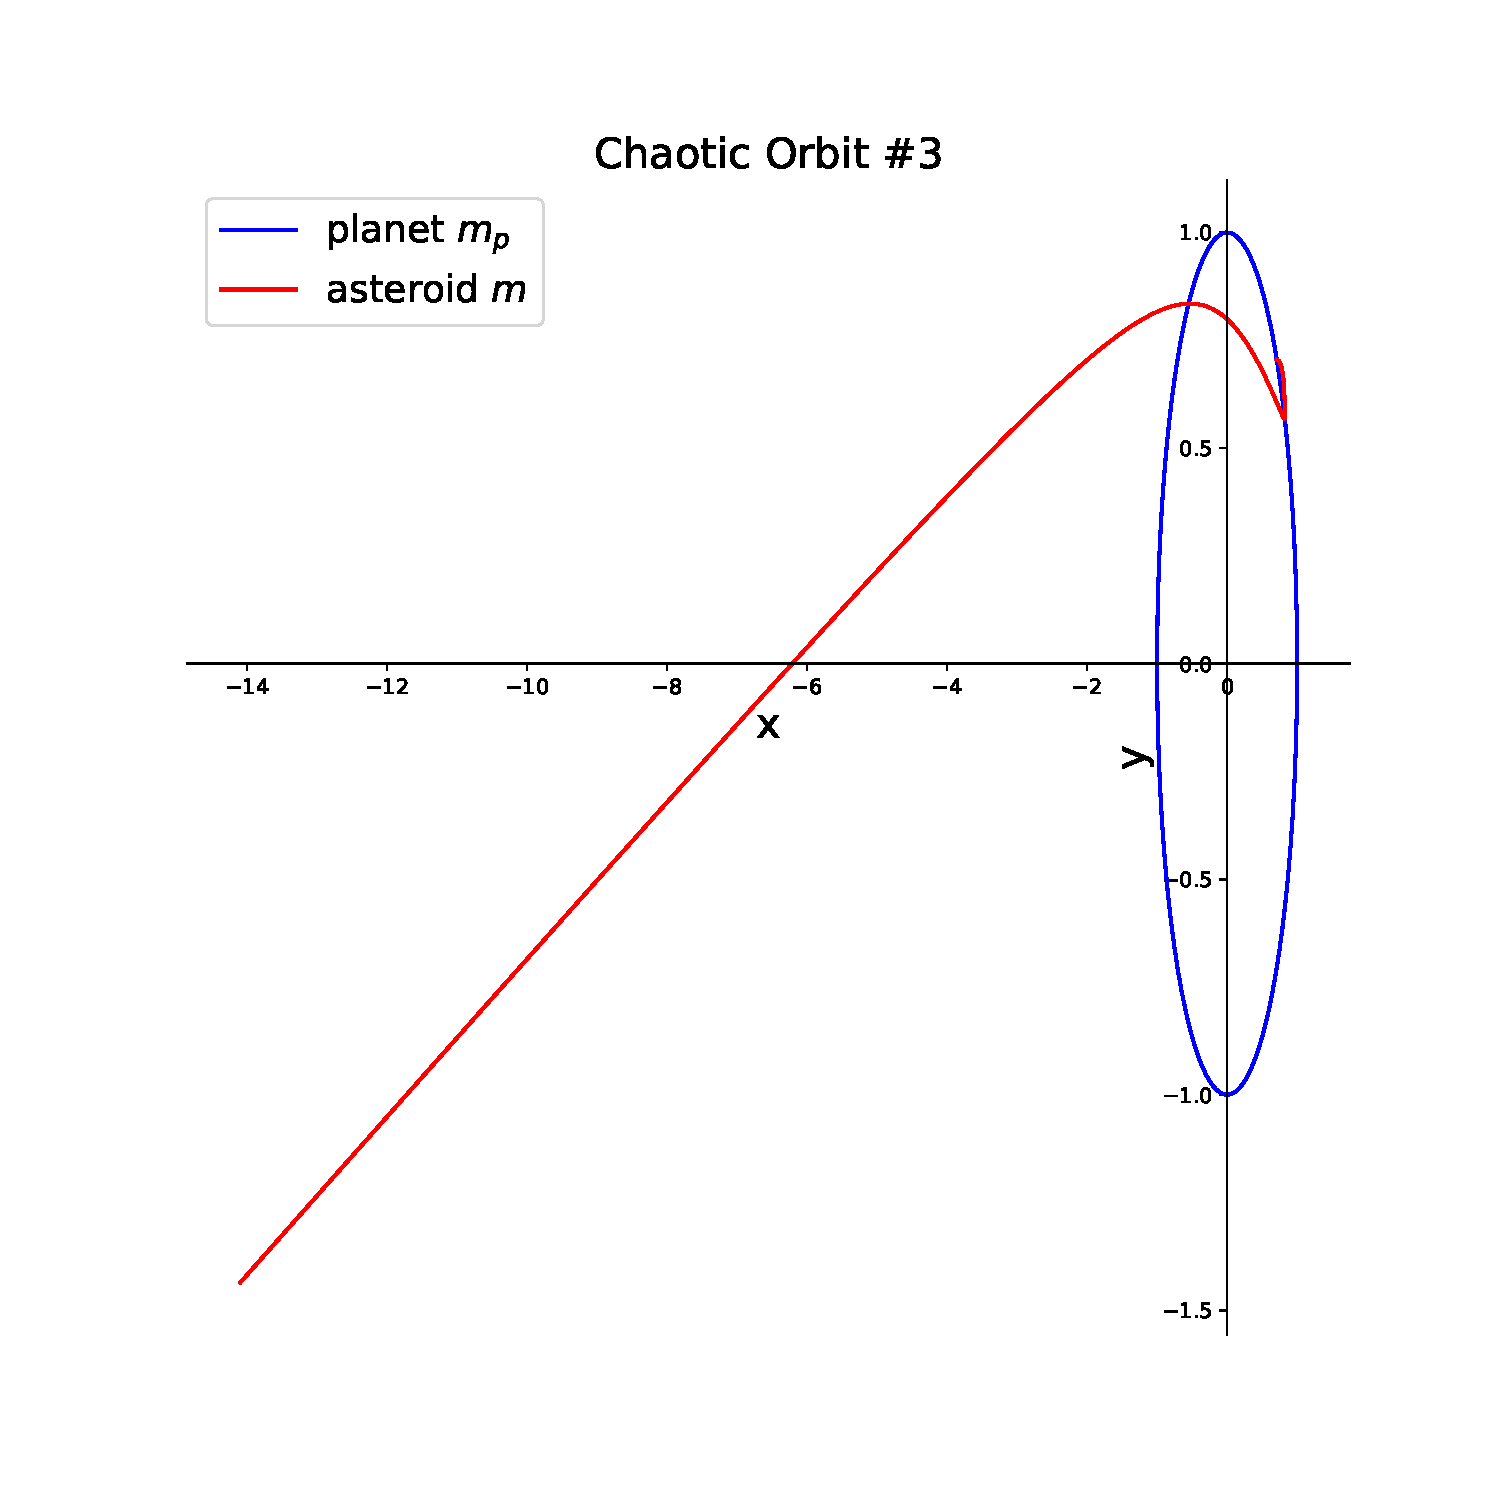
\includegraphics[width=\linewidth]{orbit3.pdf}
  \caption{the planet is orbiting the sun in an circular path, and the asteroid is moving away from the sun first, after reaching a certain distance, it turns to the left and starts moving straight.}
  \label{fig:5}
\end{subfigure}\hfil % <-- added

\label{restricted three-body images}
\end{figure}

The above six images are the results for each of the given initial conditions shown in the file $\textit{Restricted Three Body Problem 2D}$ provided. We can observe the simplest situations of both the planet and the asteroid are orbiting in a circular path, and the model of the sun, earth and the moon where the earth is moving around the sun and the moon is orbiting the earth. The last three images are examples of the asteroid flying away from the system, which can be considered to be chaotic.



\subsection{Equations of Motion $\&$ Numerical Solutions}

In this section, we will explore the nature and the numerical solutions behind a unrestricted three body problem, where the masses of the three object are similar, and the path of them are not restricted either. Solutions of this problem require that future and past motions of the bodies be uniquely determined based solely on their present positions and velocities. Using the similar ideas in the previous section, we can analyze the forces on one of the object, and apply the rules analogously to the other two objects.

For convenience and clearness, we name the three objects the Sun, the Earth and the Moon (not necessarily related to them), and we use $m_s$, $m_e$ and $m_m$  denote the mass of the Sun, the mass of the Earth and the mass of the moon respectively. We first analyze the force acting on the Sun and its position. Since the net force acting on each of the three objects are the gravitational forces exerted by the other two objects, 
\begin{align*}
    \mathbf{F}_{sun} 
    & = m_s \cdot \mathbf{a}_s \\
    & = \frac{G \left( m_s \right) \left( m_e \right)}{r_{se}^2} \left( \frac{\mathbf{r}_{se}}{\left| r_{se} \right|} \right) - \frac{G \left( m_s \right) \left( m_m \right)}{r_{ms}^2} \left( \frac{\mathbf{r}_{ms}}{\left| r_{ms} \right|} \right). \tag{71}
\end{align*}
Notice how the direction of the force plays an important role in our calculations and analysis. Therefore, the acceleration of the Sun, or the second derivative of the position of the Sun 
\begin{align*}
    a_s
    & = \frac{d^2 r}{d t^2} \\
    & = \frac{G \left( m_e \right) \left( \mathbf{r}_{se} \right)}{r_{se}^3} - \frac{G \left( m_m \right) \left( \mathbf{r}_{ms} \right)}{r_{ms}^3} \tag{72}
    \label{a of the sun}
\end{align*}
Because we are dealing with 2-D three body problem, so we disregard the z-axis. We want to use $S_x$ and $S_y$ to represent the x and y coordinates of the sun; use $E_x$ and $E_y$ to represent the x and y coordinates of the Earth; and use $M_x$ and $M_y$ to represent the x and y coordinates of the Moon, respectively. As a result, decompose $a_s$ into x-components and y-components, equation (\ref{a of the sun}) would then yield us
\begin{equation}
    \begin{cases}
        \frac{d^2 S_x}{d t^2} = \frac{G (m_e) (E_x - S_x)}{\sqrt{ (E_x - S_x)^2 + (E_y - S_y)^2} ^3} - \frac{G (m_m) (S_x - M_x)}{\sqrt{ (S_x - M_x)^2 + (S_y - M_y)^2} ^3} \\
        \frac{d^2 S_y}{d t^2} = \frac{G (m_e) (E_y - S_y)}{\sqrt{ (E_x - S_x)^2 + (E_y - S_y)^2} ^3} - \frac{G (m_m) (S_y - M_y)}{\sqrt{ (S_x - M_x)^2 + (S_y - M_y)^2} ^3}
    \end{cases}
    \tag{73}
\end{equation}
In order to solve the above equations using the $\textit{odeint()}$ function in python, we need to express the expressions in a system of first order equations because non-linear second-derivative differential equations are complicated to solve. We define $V_{sx} = \frac{d S_x}{dt}$ and $V_{sy} = \frac{d S_y}{dt}$, so:
\begin{equation}
    \begin{cases}
        \frac{d V_{sx}}{d t} = \frac{G (m_e) (E_x - S_x)}{\sqrt{ (E_x - S_x)^2 + (E_y - S_y)^2} ^3} - \frac{G (m_m) (S_x - M_x)}{\sqrt{ (S_x - M_x)^2 + (S_y - M_y)^2} ^3} \\
        V_{sx} = \frac{d S_x}{dt} \\
        \frac{d V_{sy}}{d t} = \frac{G (m_e) (E_y - S_y)}{\sqrt{ (E_x - S_x)^2 + (E_y - S_y)^2} ^3} - \frac{G (m_m) (S_y - M_y)}{\sqrt{ (S_x - M_x)^2 + (S_y - M_y)^2} ^3} \\
        V_{sy} = \frac{d S_y}{dt} 
    \end{cases}
    \tag{74}
\end{equation}
Similarly, applying the same tactics, we are able to obtain the system with 12 equations:
\begin{equation}
    \begin{cases}
        \frac{d V_{sx}}{d t} = \frac{G (m_e) (E_x - S_x)}{\sqrt{ (E_x - S_x)^2 + (E_y - S_y)^2} ^3} - \frac{G (m_m) (S_x - M_x)}{\sqrt{ (S_x - M_x)^2 + (S_y - M_y)^2} ^3} \\
        V_{sx} = \frac{d S_x}{dt} \\
        \frac{d V_{sy}}{d t} = \frac{G (m_e) (E_y - S_y)}{\sqrt{ (E_x - S_x)^2 + (E_y - S_y)^2} ^3} - \frac{G (m_m) (S_y - M_y)}{\sqrt{ (S_x - M_x)^2 + (S_y - M_y)^2} ^3} \\
        V_{sy} = \frac{d S_y}{dt} \\
        
        \frac{d V_{ex}}{d t} = - \frac{G (m_s) (E_x - S_x)}{\sqrt{ (E_x - S_x)^2 + (E_y - S_y)^2} ^3} + \frac{G (m_m) (M_x - E_x)}{\sqrt{ (M_x - E_x)^2 + (M_y - E_y)^2} ^3} \\
        V_{ex} = \frac{d E_x}{dt} \\
        \frac{d V_{ey}}{d t} = - \frac{G (m_s) (E_y - S_y)}{\sqrt{ (E_x - S_x)^2 + (E_y - S_y)^2} ^3} + \frac{G (m_m) (M_y - E_y)}{\sqrt{ (M_x - E_x)^2 + (M_y - E_y)^2} ^3} \\
        V_{ey} = \frac{d E_y}{dt} \\
        
        \frac{d V_{sx}}{d t} = - \frac{G (m_e) (M_x - E_x)}{\sqrt{ (M_x - E_x)^2 + (M_y - E_y)^2} ^3} - \frac{G (m_s) (S_x - M_x)}{\sqrt{ (S_x - M_x)^2 + (S_y - M_y)^2} ^3} \\
        V_{sx} = \frac{d S_x}{dt} \\
        \frac{d V_{sy}}{d t} = - \frac{G (m_e) (M_y - E_y)}{\sqrt{ (M_x - E_x)^2 + (M_y - E_y)^2} ^3} - \frac{G (m_s) (S_y - M_y)}{\sqrt{ (S_x - M_x)^2 + (S_y - M_y)^2} ^3} \\
        V_{sy} = \frac{d S_y}{dt} 
    \end{cases}
    \tag{75}
\end{equation}
Solving for the system of first order differential equations as shown in the file $\textit{Numerical Three Body Problem 2D}$ (appendix \ref{Appendix B}), we would then obtain the following four images.

\begin{SCfigure}[25][h]
    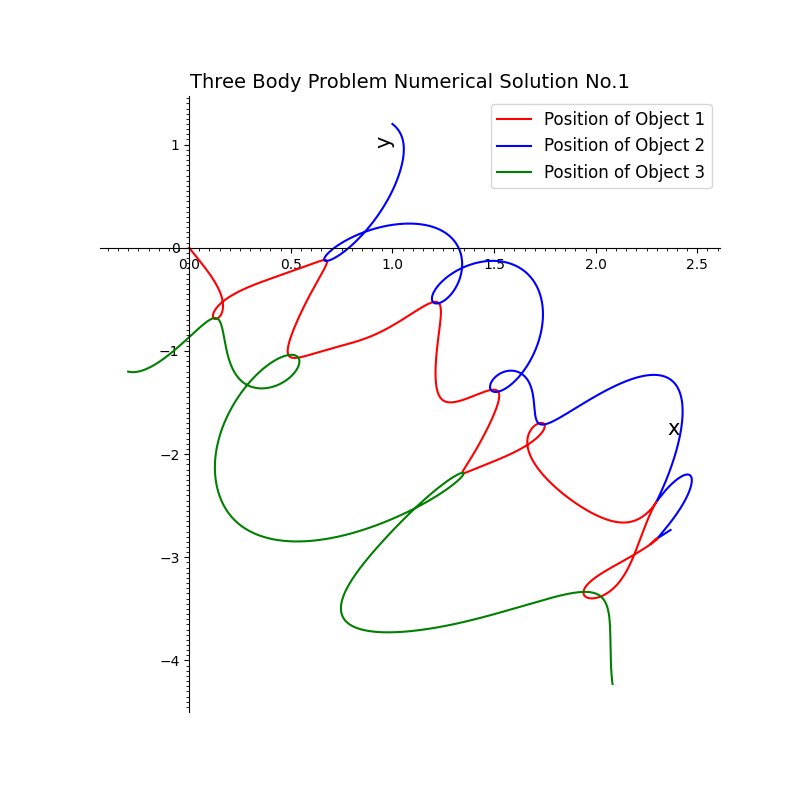
\includegraphics[width=7.5cm]{Three Body Problem Numerical Solution 1.png}
    \caption{Paths of the objects' motion in a three body problem with given initial conditions. The object 1 is interacting with each of the other objects alternatively, while the object 2 and object 3 have no intersections.}
    \label{Numerical Three Body 2D NO.1}
\end{SCfigure}

\begin{SCfigure}[25][t]
    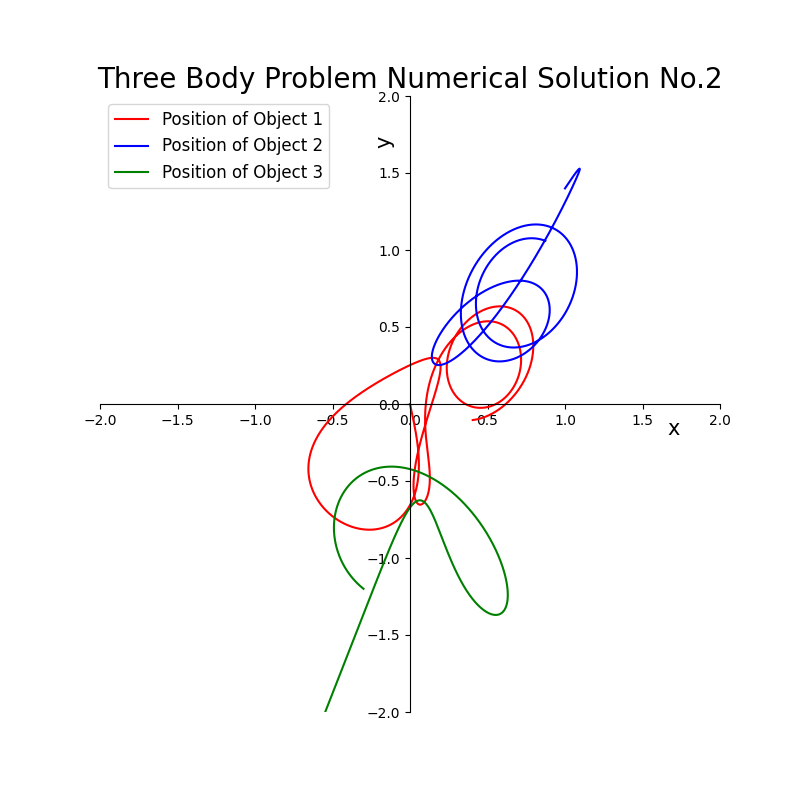
\includegraphics[width=7.2cm]{Three Body Problem Numerical Solution 2.png}
    \caption{Chaotic trajectories of the objects in a three body problem with given initial conditions}
    \label{Numerical Three Body 2D NO.2}
\end{SCfigure}

\begin{SCfigure}[25][t]
    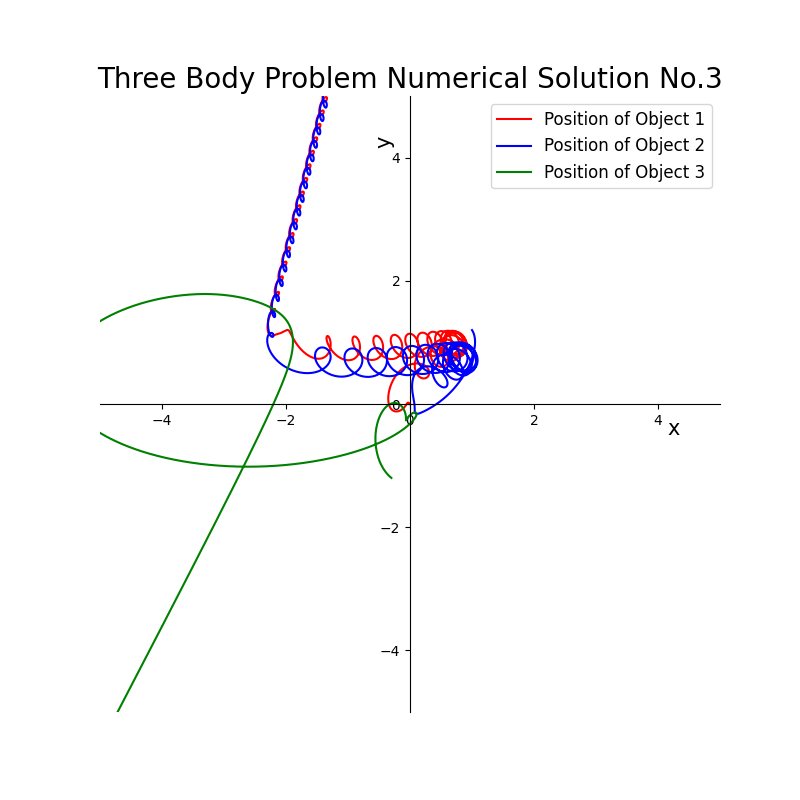
\includegraphics[width=7.2cm]{Three Body Problem Numerical Solution 3.png}
    \caption{A model of chaotic three body system with given initial conditions. At the beginning of the motion, the three objects interact with each other. After a certain point, the object 1 and object 2 interact with each other, moving away from the third object. The system then become a two body system.}
    \label{Numerical Three Body 2D NO.3}
\end{SCfigure}

\begin{SCfigure}[25][!htb]
    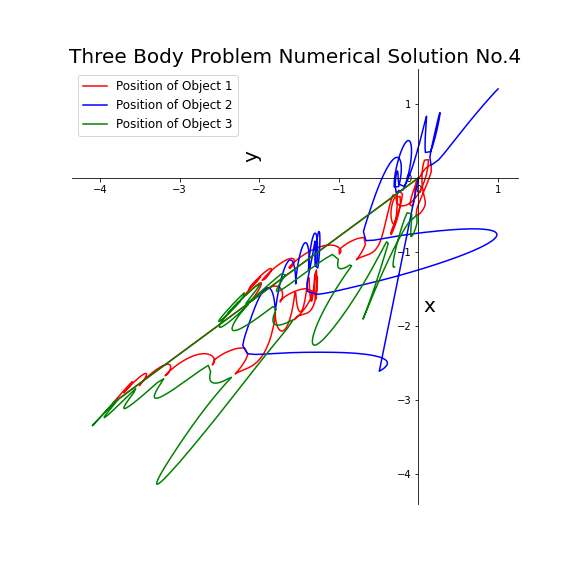
\includegraphics[width=7.2cm]{Three Body Problem Numerical Solution 4.png}
    \caption{Another model of chaotic three body system with given initial conditions, the three objects in the system are intertwining gravitationally with each other. The motions of any objects in the system are unpredictable.}
    \label{Numerical Three Body 2D NO.4}
\end{SCfigure}


\section{Conclusion}
In this project, we have showed, explained, and derived Kepler's Laws of Planetary Motion. We have showed the transform between Cartesian plane coordinates to polar coordinates, in order to solved the two-body problem for its numerical solutions, and derived the possible conics in a two-body system. We have viewed and solved for restricted three-body problem and unrestricted three-body problem in which three spherical (or point) masses interact with each other only through gravitational interactions described by Newton’s theory of gravity. 

The appealing nature and the intriguing analysis and calculations behind the problem attracts me in the first sight. The concepts, knowledge and understandings I gained in this project is significant and meaningful for me, which has also developed my interests in diverse areas such as astrophysics and computer science. 


\section{Appendix}

\subsection{Appendix A}
\label{Appendix A}

A fragment of the codes used to solve the restricted three-body problem using function $\textit{odeint()}$.

\begin{figure}[!htb]
    \centering
    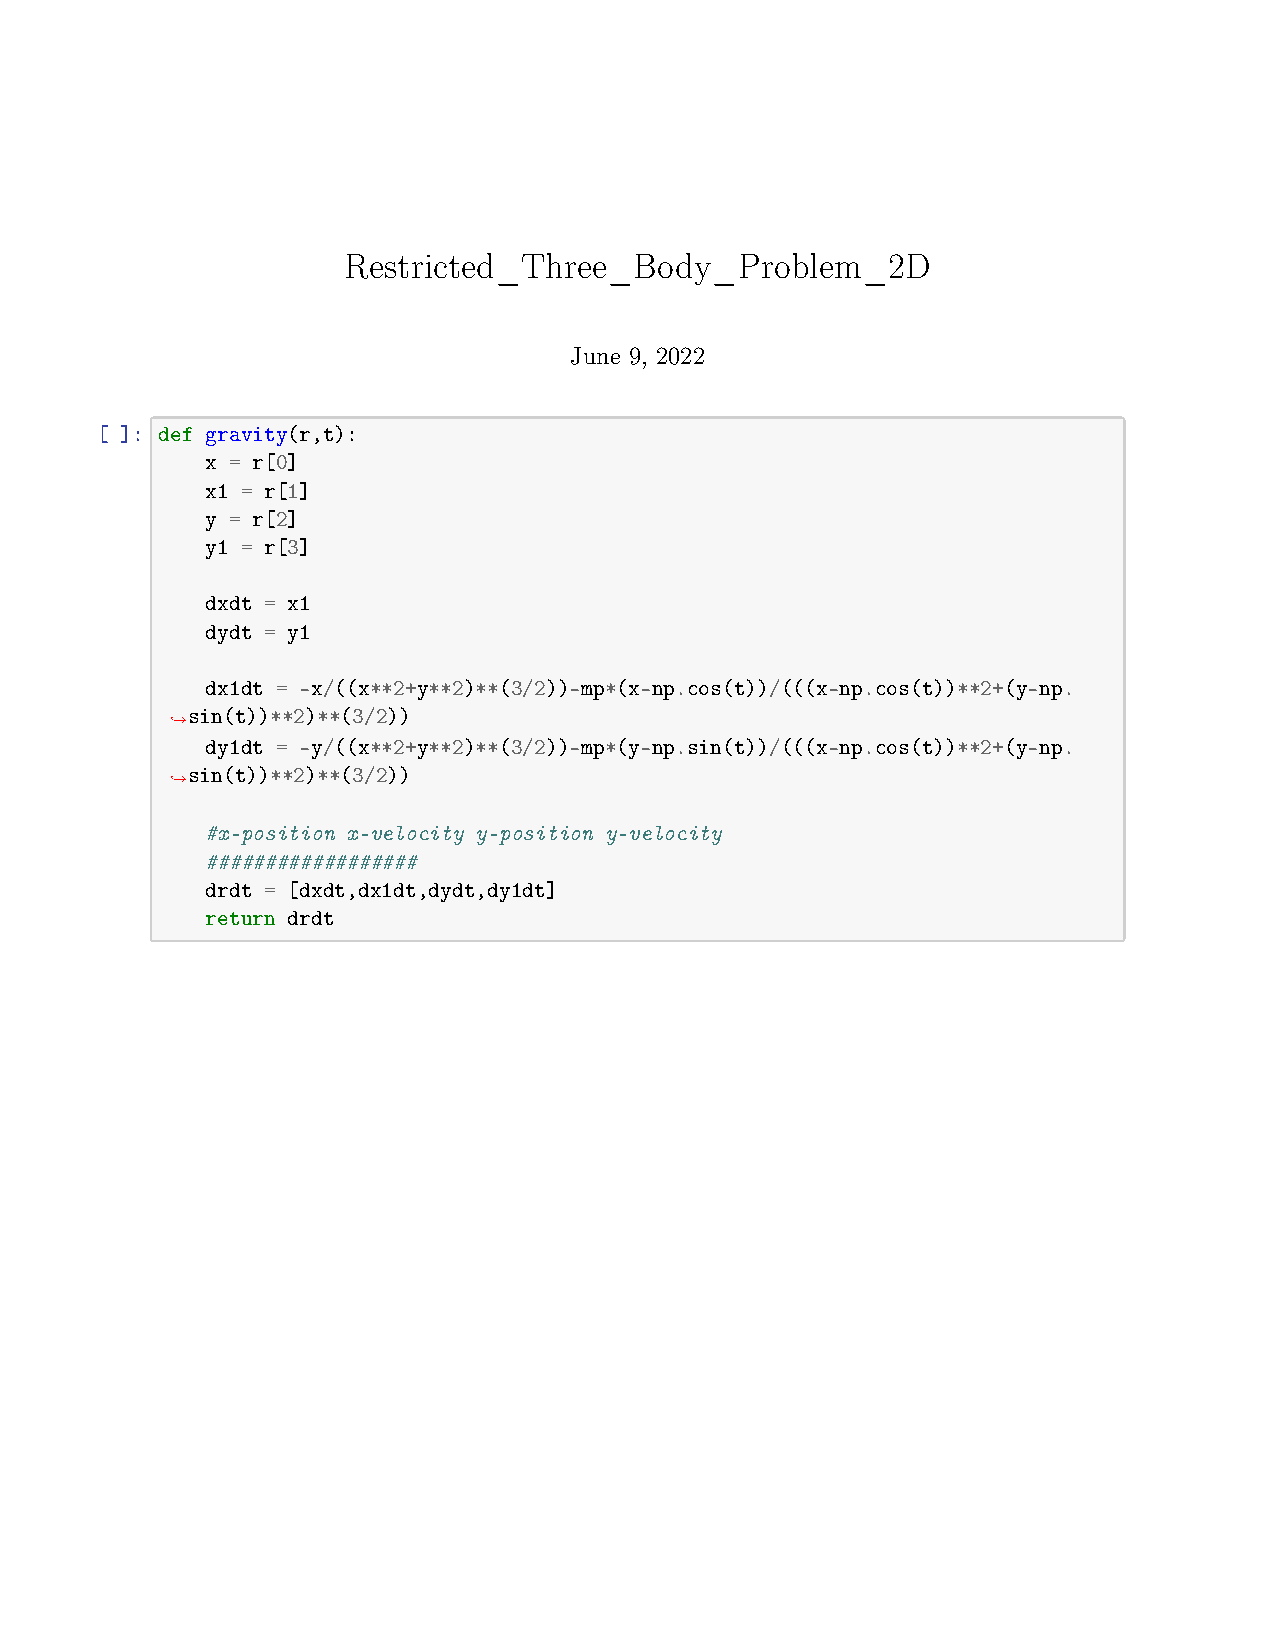
\includegraphics[width=0.75\textwidth]{RestrictedThreeBodyProblem2D.pdf}
    \caption{Portion of the codes used to find solutions for restricted three body problem}
\end{figure}

\subsection{Appendix B}
\label{Appendix B}

A fragment of the codes used to get the numerical solutions for three-body problem using function $\textit{odeint()}$.

\begin{figure}[!htb]
    \centering
    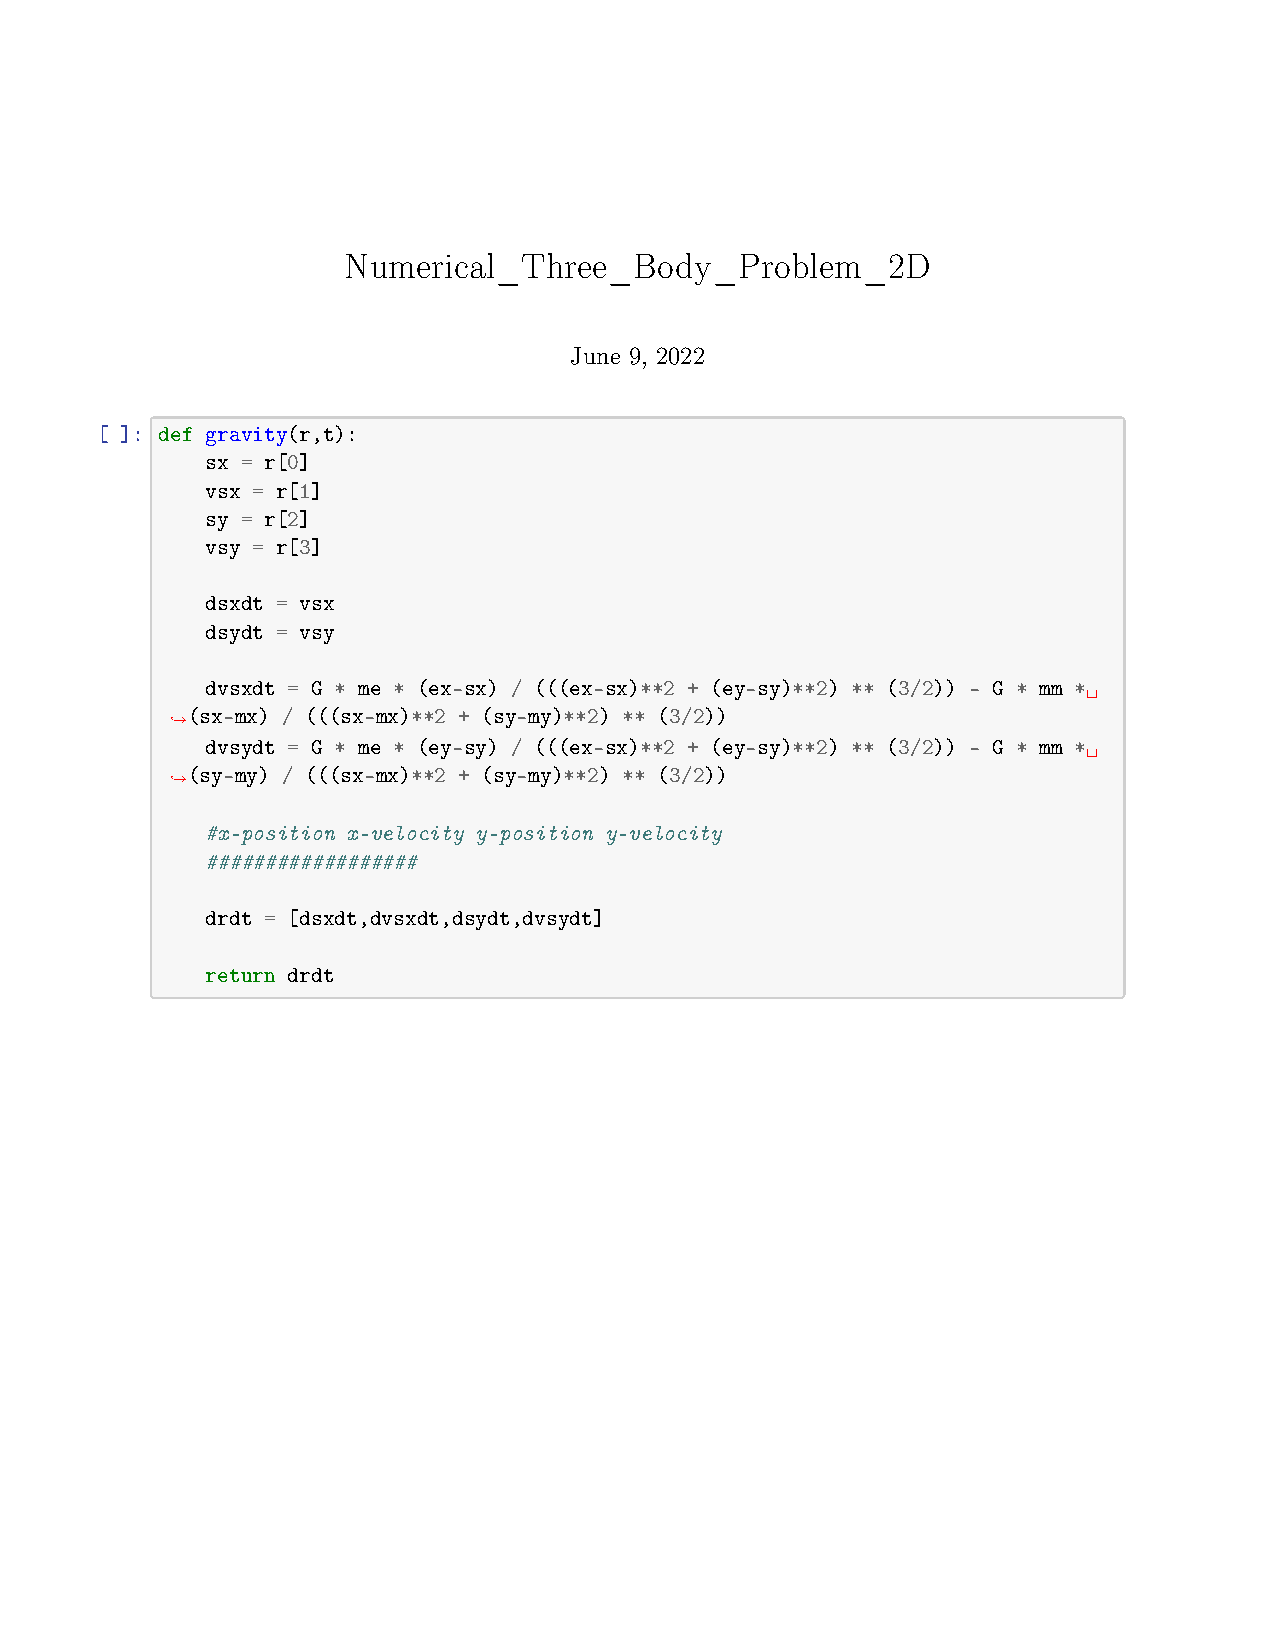
\includegraphics[width=0.75\textwidth]{NumericalThreeBodyProblem2D.pdf}
    \caption{Portion of the codes used to find numerical solutions for unrestricted three body problem}
\end{figure}










\newpage
\bibliography{main}
\end{document}
